\documentclass[final,12pt]{colt2018}

% The following packages will be automatically loaded:
% amsmath, amssymb, natbib, graphicx, url, algorithm2e

\usepackage{amsbsy,amsfonts,dsfont,fullpage,units}
\usepackage{graphicx}
\usepackage{caption}
\usepackage{multirow}
\usepackage{subcaption}
%\usepackage{subfig}
%\usepackage{epsfig}
\usepackage{float}
\usepackage{color}
\usepackage{cases}
\usepackage{xcolor}
\usepackage[normalem]{ulem}
\usepackage{times}
\usepackage{thmtools}
\usepackage{layouts}


%\usepackage{algorithm}
\usepackage{algorithmic}
\usepackage{algorithm2e}
\usepackage{tikz}
\usetikzlibrary{calc,shapes}
%\usepackage[round]{natbib}
\usepackage{hyperref}
\usepackage{dsfont}
\usepackage{textcomp}


\newtheorem{claim}{Claim}
\newtheorem*{claim*}{Claim}
%\newtheorem{corollary}{Corollary}[section]
%\newtheorem{assumption}{Assumption}[section]
%\newtheorem{lemma}{Lemma}[section]
%\newtheorem{proposition}{Proposition}[section]
%\newtheorem{theorem}{Theorem}[section]
%\newtheorem{fact}{Fact}[section]
%\theoremstyle{definition}
%\newtheorem{condition}{Condition}[section]
%\newtheorem{definition}{Definition}
%\newtheorem{example}{Example}
%\theoremstyle{remark}
%\newtheorem{remark}{Remark}

\graphicspath{ {diagrams/} }

\newcommand{\defeq}{\mathrel{\mathop:}=}
\newcommand{\red}[1]{{\color{black} #1}}
\newcommand{\praneeth}[1]{{\color{blue} PN:#1}}
\newcommand{\gd}{GD}
\newcommand{\pgd}{PGD}
\newcommand{\pagd}{PAGD}
\newcommand{\nag}{AGD}
\newcommand{\fstar}{f^*}
\newcommand{\xstar}{\x^*}
\newcommand{\nce}{NCE}

\newcommand{\vect}[1]{\ensuremath{\mathbf{#1}}}
\newcommand{\mat}[1]{\ensuremath{\mathbf{#1}}}
\newcommand{\dd}{\mathrm{d}}
\newcommand{\grad}{\nabla}
\newcommand{\hess}{\nabla^2}
\newcommand{\argmin}{\mathop{\rm argmin}}
\newcommand{\argmax}{\mathop{\rm argmax}}

\newcommand{\abs}[1]{\left|{#1}\right|}
\newcommand{\norm}[1]{\left\|{#1}\right\|}
\newcommand{\order}[1]{O\left({#1}\right)}
\newcommand{\otheta}[1]{\Theta\left({#1}\right)}
\newcommand{\otilde}[1]{\widetilde{O}\left({#1}\right)}
\newcommand{\omtilde}[1]{\widetilde{\Omega}\left({#1}\right)}
\newcommand{\fnorm}[1]{\left\|{#1}\right\|_{\text{F}}}
\newcommand{\spnorm}[2]{\left\| {#1} \right\|_{\text{S}({#2})}}
\newcommand{\sigmin}{\sigma_{\min}}
\newcommand{\tr}{\text{tr}}
\renewcommand{\det}{\text{det}}
\newcommand{\rank}{\text{rank}}
\newcommand{\logdet}{\text{logdet}}
\newcommand{\trans}{^{\top}}
\newcommand{\poly}{\text{poly}}
\newcommand{\polylog}{\text{polylog}}
\newcommand{\st}{\text{s.t.~}}
\newcommand{\proj}{\mathcal{P}}
\newcommand{\projII}{\mathcal{P}_{\parallel}}
\newcommand{\projT}{\mathcal{P}_{\perp}}

\newcommand{\Bcal}{\mathcal{B}}
\newcommand{\Z}{\mathbb{Z}}
\newcommand{\N}{\mathbb{N}}
\newcommand{\R}{\mathbb{R}}
\newcommand{\C}{\mathbb{C}}
\newcommand{\E}{\mathbb{E}}
\newcommand{\Var}{\text{Var}}

\newcommand{\iol}{improve or localize}

\newcommand{\fracpar}[2]{\frac{\partial #1}{\partial  #2}}

\newcommand{\A}{\mat{A}}
\newcommand{\B}{\mat{B}}
\newcommand{\Q}{\mat{Q}}


\newcommand{\I}{\mat{I}}
\newcommand{\M}{\mat{M}}
\newcommand{\D}{\mat{D}}
\newcommand{\U}{\mat{U}}
\newcommand{\V}{\mat{V}}
\newcommand{\W}{\mat{W}}
\newcommand{\X}{\mat{X}}
\newcommand{\Y}{\mat{Y}}
\newcommand{\mSigma}{\mat{\Sigma}}
\newcommand{\mLambda}{\mat{\Lambda}}
\newcommand{\e}{\vect{e}}
\renewcommand{\u}{\vect{u}}
\renewcommand{\v}{\vect{v}}
\newcommand{\w}{\vect{w}}
\newcommand{\x}{\vect{x}}
\newcommand{\y}{\vect{y}}
\newcommand{\z}{\vect{z}}
\newcommand{\fI}{\mathfrak{I}}
\newcommand{\fS}{\mathfrak{S}}
\newcommand{\fE}{\mathfrak{E}}
\newcommand{\fF}{\mathfrak{F}}

\renewcommand{\L}{\mathcal{L}}
\renewcommand{\H}{\mathcal{H}}

\newcommand{\cn}{\kappa}
\newcommand{\nn}{\nonumber}


\newcommand{\Hess}{\nabla^2}
\newcommand{\tlO}{\tilde{O}}
\newcommand{\tlOmega}{\tilde{\Omega}}
\newcommand{\iprod}[2]{\langle #1, #2 \rangle}

% \newcommand{\M}{\mat{M}}
% \newcommand\Mmh{\mat{M}^{-1/2}}
% \newcommand{\A}{\mat{A}}
% \newcommand{\B}{\mat{B}}
% \newcommand{\C}{\mat{C}}
% \newcommand{\Et}[1][t]{\mat{E_{#1}}}
% \newcommand{\Etp}{\Et[t+1]}
% \newcommand{\Errt}[1][t]{\mat{\bigtriangleup_{#1}}}
% \newcommand\cnM{\kappa}
% \newcommand{\cn}[1]{\kappa\left(#1\right)}
% \newcommand\X{\mat{X}}
% \newcommand\fstar{f_*}
% \newcommand\Xt[1][t]{\mat{X_{#1}}}
% \newcommand\ut[1][t]{{u_{#1}}}
% \newcommand\Xtinv{\inv{\Xt}}
% \newcommand\Xtp{\mat{X_{t+1}}}
% \newcommand\Xtpinv{\inv{\left(\mat{X_{t+1}}\right)}}
% \newcommand\U{\mat{U}}
% \newcommand\UTr{\trans{\mat{U}}}
% \newcommand{\Ut}[1][t]{\mat{U_{#1}}}
% \newcommand{\Utinv}{\inv{\Ut}}
% \newcommand{\UtTr}[1][t]{\trans{\mat{U_{#1}}}}
% \newcommand\Utp{\mat{U_{t+1}}}
% \newcommand\UtpTr{\trans{\mat{U}_{t+1}}}
% \newcommand\Utptild{\mat{\widetilde{U}_{t+1}}}
% \newcommand\Us{\mat{U^*}}
% \newcommand\UsTr{\trans{\mat{U^*}}}
% \newcommand{\Sigs}{\mat{\Sigma}}
% \newcommand{\Sigsmh}{\Sigs^{-1/2}}
% \newcommand{\eye}{\mat{I}}
% \newcommand{\twonormbound}{\left(4+\DPhi{\M}{\Xt[0]}\right)\twonorm{\M}}
% \newcommand{\lamj}{\lambda_j}

% \renewcommand\u{\vect{u}}
% \newcommand\uTr{\trans{\vect{u}}}
% \renewcommand\v{\vect{v}}
% \newcommand\vTr{\trans{\vect{v}}}
% \newcommand\w{\vect{w}}
% \newcommand\wTr{\trans{\vect{w}}}
% \newcommand\wperp{\vect{w}_{\perp}}
% \newcommand\wperpTr{\trans{\vect{w}_{\perp}}}
% \newcommand\wj{\vect{w_j}}
% \newcommand\vj{\vect{v_j}}
% \newcommand\wjTr{\trans{\vect{w_j}}}
% \newcommand\vjTr{\trans{\vect{v_j}}}

% \newcommand{\DPhi}[2]{\ensuremath{D_{\Phi}\left(#1,#2\right)}}
% \newcommand\matmult{{\omega}}


\newcommand{\todo}[1]{{\color{red}{TODO:#1}}}
\definecolor{WildStrawberry}{RGB}{255,67,164}

\newcommand{\nishanth}[1]{{\color{blue}{ND: #1}}}
\newcommand{\nick}[1]{{\color{WildStrawberry}{NG: #1}}}
\newcommand{\costis}[1]{{\color{red}{CD: #1}}}
\newcommand{\corrected}[1]{{\color{ForestGreen}{\sout{#1}}}}
\renewcommand{\circ}{\cdot}

\title{Testing Symmetric Markov Chains From a Single Trajectory}
%\title{Testing Markov Chains: Application to Riffle Shuffle}
%\title{Testing from a {\em Single Sample}:\\Markov chain goodness-of-fit and the riffle shuffle}
%\title{Testing from {\em One} Sample: Is the casino really using a riffle shuffle?}

%\date{}


\coltauthor {\Name{Constantinos Daskalakis} \Email{costis@mit.edu}\\
\thanks{Supported by a Microsoft Research Faculty Fellowship, and NSF Award CCF-1551875, CCF-1617730 and CCF-1650733.}\\
\addr EECS, MIT 
\AND
\Name{Nishanth Dikkala} \Email{nishanthd@csail.mit.edu}\\
\thanks{Supported by NSF Award CCF-1551875, CCF-1617730 and CCF-1650733.}\\
\addr EECS, MIT 
\AND
\Name{Nick Gravin} \Email{nikolai@mail.shufe.edu.cn} \\
\thanks{Supported by NSF Award CCF-1551875, CCF-1617730 and CCF-1650733.}\\
\addr ITCS, SHUFE
}








\begin{document}
%\date{}

\maketitle

We present preconditioned stochastic gradient descent (SGD) algorithms for the $\ell_1$ minimization problem $\min_{\xx}\|\AA \xx - \bb\|_1$ in the overdetermined case, where there are far more constraints than variables. Specifically, we have $\AA \in \R^{n \times d}$ for $n \gg d$. Commonly known as the Least Absolute Deviations problem, $\ell_1$ regression can be used to solve many important combinatorial problems, such as minimum cut and shortest path. SGD-based algorithms are appealing for their simplicity and practical efficiency.
% Our algorithms precondition the matrix $\AA$ and then solve the problem for the resulting matrix $\tilde{\AA}$ using gradient descent techniques.
Our primary insight is that careful preprocessing can yield preconditioned matrices $\tilde{\AA}$ with strong properties (besides good condition number and low-dimension) that allow for faster convergence of gradient descent. In particular, we precondition using Lewis weights to obtain an isotropic matrix with fewer rows and strong upper bounds on all row norms. We leverage these conditions to find a good initialization, which we use along with recent smoothing reductions and accelerated stochastic gradient descent algorithms to achieve $\epsilon$ relative error in $\Otil(nnz(\AA) + d^{2.5} \epsilon^{-2})$ time with high probability, where $nnz(\AA)$ is the number of non-zeros in $\AA$. This improves over the previous best result using gradient descent for $\ell_1$ regression. We also match the best known running times for interior point methods in several settings.

Finally, we also show that if our original matrix $\AA$ is approximately isotropic and the row norms are approximately equal, we can give an algorithm that avoids using fast matrix multiplication and obtains a running time of $\Otil(nnz(\AA) + s d^{1.5}\epsilon^{-2} + d^2\epsilon^{-2})$, where $s$ is the maximum number of non-zeros in a row of $\AA$. In this setting, we beat the best interior point methods for certain parameter regimes.


%We consider the $\ell_1$ minimization problem $\min_{\xx}||\AA \xx - \bb||_1$ in the overconstrained case, where there are far more constraints than variables. More specifically, we have $\AA \in \R^{n \times d}$ for $n \gg d$. By using Lewis Weights preconditioning on $\AA$ and a careful initialization, we show that a standard stochastic gradient descent algorithm achieves $\epsilon$ relative error in about $nnz(\AA) +  d^3\epsilon^{-2}$ time with high probability. If we leverage smoothing reductions in \cite{AllenZhuH16} and the accelerated stochastic gradient descent algorithms in \cite{AllenZhu17}, we can achieve a running time of about $nnz(\AA) + d^{2.5}\epsilon^{-2}$ with the same guarantees. Both of these running times improve over the previous results in \cite{YangCRM16} and the latter result is comparable to the best known running times for interior point methods \cite{LeeS15}.
%
%The key idea will be to use our preconditioning to restrict our consideration to matrices $\AA$ such that $\AA^T\AA = \II$ and every row norm of $\AA$ is upper bounded by $O(\sqrt{d/n})$. \cite{cohenpeng} show that sampling $\AA$ with Lewis weights takes about $nnz(\AA) +d^{\omega}$ time and approximately preserves the minimization problem. Moreover, we can assume $n\le O(d\epsilon^{-2}\log n)$ for the sampled matrix. We then prove that all leverage scores of the sampled matrix are approximately equal. Since rotations preserve leverage scores, we can then rotate our sampled matrix to ensure that our desired properties are met in about $d^{\omega}\epsilon^{-2}$ time.
%
%Finally, we also show that if our original matrix $\AA$ is such that $\AA^T\AA \approx \II$ and the row norms of $\AA$ are bounded, we can avoid using fast matrix multiplication and prove a running time of about $nnz(\AA) + s d^{1.5}\epsilon^{-2}$, where $s$ is the maximum number of non-zeros in a row of $\AA$.

%Consequently, we will be able to restrict our consideration to matrices $A$ such that $A^TA \approx I$, and all row norms are equal, which is to say $||A_{i,:}||_2 = \sqrt{\frac{d}{n}}$ for all $i$.
%
%With a careful choice of our initial $x$, we show that standard gradient descent and stochastic gradient descent algorithms under these further assumptions only require $O(\frac{d}{\epsilon^2})$ and $O(\frac{d^2}{\epsilon^2})$ iterations, respectively, to achieve $\epsilon$ relative error with respect to the minimum objective value. Accordingly, these methods each achieve respective total runtime of $O(\frac{md}{\epsilon^2})$ and $O(\frac{d^3}{\epsilon^2})$, along with an $O(m)$ preconditioning cost, improving over the previous results in \cite{MahoneySGD}.
%
%We further examine the consequences of our assumptions when combined with smoothing reductions in [cite] and accelerated gradient descent techniques in [cite,cite]. As a result we are able to further improve the running times to $O(\frac{md}{\epsilon})$ and $O(dn\log{1/\epsilon} + \frac{d^2\sqrt{n}}{\epsilon})$.
%
%Random sampling $d\epsilon^{-2}\log{d}$ rows of $A$ will only incur error $\epsilon$ and reduces the latter running time to $O(\frac{d^{2.5}\log{d}}{\epsilon^2})$, which is then comparable to interior point methods of [cite]



\thispagestyle{empty}
\addtocounter{page}{-1}
\newpage
\section{Introduction}
\label{sec:intro}
% !TeX root = main.tex
\section{Introduction}
\label{sec:intro}
Generative models are often trained in an unsupervised fashion, fitting a model $q$ to a set of observed data $x_P \subseteq X$ drawn iid from some true distribution $p$ on $x\in X$. Now, of course $p$ may not exactly belong to family $Q$ of probability distributions being fit, whether $Q$ consists of Gaussians mixture models, Markov models, or even neural networks of bounded size. We first discuss the limitations of generative modeling without feedback, and then discuss our model and results.

%\subsection{Limitations of Generative Modeling from Positive Examples Alone}
Consider fitting a generative model on a text corpus consisting partly of poetry written by four-year-olds and partly of mathematical publications from the {\em Annals of Mathematics}. Suppose that learning to generate a poem that looks like it was written by a child was easier than learning to generate a novel mathematical article with a correct, nontrivial statement. If the generative model pays a high price for generating unrealistic examples, then it may be better off learning to generate children's poetry than mathematical publications. However, without negative feedback, it may be difficult for a neural network or any other model to know that the mathematical articles it is generating are stylistically similar to the mathematical publications but do not contain valid proofs.\footnote{This is excluding clearly fake articles published without proper review in lower-tier venues \citep{LabbeL13}.} 

As a simpler example, the classic Markovian ``trigram model'' of natural language assigns each word a fixed probability conditioned only on the previous two words. Prior to recent advances in deep learning, for decades the trigram model and its variant were the workhorses of language modeling, assigning much greater likelihood to natural language corpora than numerous linguistically motivated grammars and other attempts \citep{Rosenfeld00}. However, text sampled from a trigram is typically nonsensical, e.g., the following text was randomly generated from a trigram model fit on a corpus of text from the Wall Street Journal \citep{JurafskyM09}:
\begin{quote}
They also point to ninety nine point six billion dollars from two hundred
four oh six three percent of the rates of interest stores as Mexico and
gram Brazil on market conditions. 
\end{quote}

In some applications, like text compression using a language model \citep{WittenNC87}, maximizing likelihood is equivalent to optimizing compression. However, in many  applications involving generation, such nonsense is costly and unacceptable. Now, of course it is possible to always generate valid data by returning random training examples, but this is simply overfitting and not learning. Alternatively, one could incorporate human-in-the-loop feedback such as through crowdsourcing, into the generative model to determine what is a valid, plausible sentence.

In some domains, validity could be determined automatically. Consider a Markovian model of a well-defined concept such as mathematical formulas that compile in \LaTeX{}. Now, consider a $n$-gram Markovian character model which the probability of each subsequent character is determined by the previous $n$ characters. For instance, the expression \$\{2+\{x-y\}\$ is invalid in \LaTeX{} due to mismatched braces. For this problem, a \LaTeX{} compiler may serve as a validity oracle. Various $n$-gram models can be fit which only generate valid formulas. To address mismatched braces, for example, one such model would ensure that it always closed braces within $n$ characters of opening, and had no nested braces. While an $n$-gram model will not perfectly model the true distribution over valid \LaTeX{} formulas, for certain generative purposes one may prefer an $n$-gram model that generates valid formulas over one that assigns greater likelihood to the training data but generates invalid formulas. 

Figure \ref{fig:rectangle} illustrates a simple case of learning a rectangle model for data which is not uniform over a rectangle. A maximum likelihood model would necessarily be the smallest rectangle containing all the data, but most examples generated from this distribution may be invalid. Instead a smaller rectangle, as illustrated in the figure, may be desired.

\begin{figure}[h]\label{fig:rectangle}
\centering
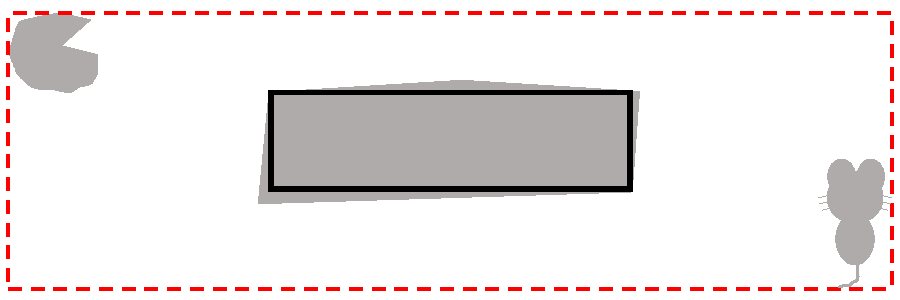
\includegraphics[width=3in]{fig.pdf}
\caption{Example where the underlying distribution $p$ is uniform over the (gray) valid regions. The solid rectangle maximizes our objective since it does not output nonsense (is supported only within the grey matter) and is closest to the $p$ (covers the maximum amount of grey matter). In contrast, the standard maximum likelihood (dashed red) rectangle must fully contain the observed samples, thus generating invalid points most of the time.  }
\end{figure}

Motivated by these observations, we evaluate a generative model $q$ on two axes. First is {\em coverage}, which is related to the probability assigned to future examples drawn from the true distribution $p$. Second is {\em validity}, defined as the probability that random examples generated from $q$ meet some validity requirement. Formally, we measure coverage in terms of a bounded {\em loss}:
$$\Loss(p,q)=\E_{x \sim p}[L(q_x)],$$
where $L:[0,1]\rightarrow [0,M]$ is a bounded decreasing function such as the capped log-loss $L(q_x)=\min(M, \log 1/q_x)$. % or $L(q_x)=\log 1/(q_x+\exp(-M))$. 
A bounded loss has the advantages of being efficiently estimable, and also it enables a model to assign 0 probability to one example (e.g., an outlier or error) if it greatly increases the likelihood of all other data. Validity is defined with respect to a set $V \subseteq X$, and $q(V)$ is the probability that a random example generated from $q$ lies within $V$. 

Clearly, there is a tradeoff between coverage and validity. We first focus on the case of (near) perfect validity. A Valid Generative Modeling (VGM) algorithm if it outputs, for a family of distributions $Q$ over $X$, if it outputs $\hat{q}$ with (nearly) perfect validity and whose loss is nearly as good as the loss of the best valid $q\in Q$. More precisely, $A$ is a VGM learner of $Q$ if for any nonempty valid subset $V \subseteq X$, any probability distribution $p$ over $V$, and any $\eps>0$, $A$ uses $n$ random samples from $p$ and makes $m$ membership oracle calls to $V$ and outputs a distribution $\hat{q}$ such that, $$\Loss(p, \hat{q}) \leq \min_{q \in Q: q(V)=1}\Loss(p,q) + \eps ~\text{ and }~\hat{q}(V)\geq 1-\eps.$$ 
We aim for our learner to be sample and query efficient, requiring that $n$ and $m$ are polynomial in $M, 1/\eps$ and a measure of complexity of our distribution class $Q$.
Furthermore, we would like our algorithms to be computationally efficient, with a runtime polynomial in the size of the data, namely the $n + m$ training examples. 
A more formal description of the problem is available in Section~\ref{sec:problem}.

$A$ is said to be {\em proper} if it always outputs $\hat{q}\in Q$ and {\em improper} otherwise.
In Section~\ref{sec:impossibility}, we first show that efficient proper learning for VGM is impossible. This is an information-theoretic result, meaning that even given infinite runtime and positive samples, one still cannot solve the VGM problem. Interestingly, this is different from binary classification, where it is possible to statistically learn from iid examples without a membership oracle.

Our first main positive result is an efficient (improper) learner for VGM. The algorithm relies on a subroutine that solves the following {\em Generative Modeling with Negatives} (GMN) problem: given sets $X_P, X_N \subset X$ of positive and negative examples, find the probability distribution $q \in Q$ which minimizes $\sum_{x \in X_P} L(q(x))$ subject to the constraint that $q(X_N)=0$. For simplicity, we present our algorithm for the case that the distribution family $Q$ is finite, giving sample and query complexity bounds that are logarithmic in terms of $|Q|$. However, as we show in Section~\ref{sec:infinite-families}, all of our results extend to infinite families $Q$. It follows that if one has a computationally efficient algorithm for the GMN problem for a distribution family $Q$, then our reduction gives a computationally efficient VGM learning algorithm for $Q$.

Our second positive result is an algorithm that minimizes $\Loss(p,q)$ subject to a relaxed validity constraint comparing against the optimal distribution that has validity $q(V)$ at least $1-\alpha$ for some $\alpha>0$. We show in Section~\ref{sec:partial-validity} that even in this more general setting, it is possible to obtain an algorithm that is statistically efficient but may not be computationally efficient. An important open question is whether there exists a computationally efficient algorithm for this problem when given access to an optimization oracle, as was the case for our algorithm for VGM.

\subsection{Related Work}
\cite{KearnsMRRSS94} showed how to learn distributions from positive examples in the realizable setting, i.e., where the true distribution is assumed to belong to the class being learned. In the same sense as their work is similar to PAC learning \citet{Valiant84} of distributions, our work is like agnostic learning \citet{KearnsSS94} in which no assumption on the true distribution is made. 

Generative Adversarial Networks (GANs)~\cite{GoodfellowPMXWOCB14} are an approach for generative modeling from positive examples alone, in which a generative model is trained against a discriminator that aims to distinguish real data from generated data. In some domains, GANs have been shown to outperform other methods at generating realistic-looking examples. Several shortcomings of GANs have been observed \citet{AroraRZ18}, and GANs are still subject to the theoretical limitations we argue are inherent to any model trained without a validity oracle. 

In supervised learning, there is a rich history of learning theory with various types of queries, including membership which are not unlike our (in)validity oracle. Under various assumptions, queries have been shown to facilitate the learning of complex classes such as finite automata \citet{Angluin88} and DNFs \citet{Jackson97}. See the survey of \cite{Angluin92} for further details.  Interestingly, \cite{Feldman09} has shown that for agnostic learning, i.e., without making assumptions on the generating distribution, the addition of membership queries does not enhance what is learnable beyond random examples alone. 
Supervised learning also has a large literature around active learning, showing how the ability to query examples reduces the sample complexity of many algorithms. See the survey of \cite{Hanneke14}. Note that the aim here is typically to save examples and not to expand what is learnable.
 
More sophisticated models, e.g., involving neural networks, can mitigate the invalidity problem as they often generate more realistic natural language and have even been demonstrated to generate \LaTeX{} that nearly compiles \citep{Karpathy15} or nearly valid Wikipedia markdown. However, longer strings generated are unlikely to be valid. For example, \cite{Karpathy15} shows generated markdown which includes:
\begin{quote}
==Access to ''rap===
The current history of the BGA has been [[Vatican Oriolean Diet]], British Armenian, published in 1893.  While actualistic such conditions such as the [[Style Mark Romanians]] are still nearly not the loss.
\end{quote}

Even ignoring the mismatched quotes and equal signs, note that this example has two so-called ``red links'' to two pages that do not exist. Without checking, it was not obvious to us whether or not Wikipedia had pages titled {\em Vatican Oriolean Diet} or {\em Style Mark Romanians}. In some applications, one may or may not want to disallow red links. In the case that they are considered valid, one may seek a full generative model of what might plausibly occur inside of brackets, as the neural network has learned in this case. If they are disallowed, a model might memorize links it has seen but not generate new ones. A validity oracle can help the learner identify what it should avoid generating.

 In practice, \cite{KusnerPH17} discuss how generative models from neural networks (in particular autoencoders) often generate invalid sequences. 
\cite{JanzWPKH18} learn the validity of examples output by a generative model using oracle feedback. 


%\section{Outline}
%\label{sec:outline}
%\input{outline}

\section{Preliminaries}
\label{sec:prelim}
%!TEX root = main.tex

\section{Preliminaries}
In this section, we will review some well-known results on~\gd~and~\nag~in the strongly convex setting, 
and existing results on convergence of~\gd~to second-order stationary points. 
% The pseudocode for these algorithms is given in Algorithms~\ref{algo:gd} and~\ref{algo:AGD} respectively.

% \cnote{Show gradient descent in equation}

\subsection{Notation}
Bold upper-case letters ($\A, \B$) denote matrices and bold lower-case letters ($\x, \y$) denote vectors. 
For vectors $\norm{\cdot}$ denotes the $\ell_2$-norm. For matrices, $\norm{\cdot}$ denotes the spectral norm and $\lambda_{\min}(\cdot)$ denotes the minimum eigenvalue.
For $f: \R^d \rightarrow \R$, $\grad f(\cdot)$ and  $\hess f(\cdot)$ denote its gradient and Hessian respectively, and $f^\star$ denotes its global minimum.
% Other than Section \ref{sec:related}, 
We use $O(\cdot), \Theta(\cdot), \Omega(\cdot)$ to hide absolute constants, and $\tilde{O}(\cdot), \tilde{\Theta}(\cdot), \tilde{\Omega}(\cdot)$ to hide absolute constants and polylog factors for all problem parameters. 
% \praneeth{I think it will be cleaner to make the dependence on smoothness parameters in Table~\ref{tab:main} and edit this statement} \jccomment{Then I also need to add function value dependence, maybe too complicated to compare}.\praneeth{The issue with this is that $O()$ is not just hiding constants but also problem dependent parameters. May be mention this explicitly in the caption to the table.} 
% We let $\ball^{(d)}_\x(r)$ denote the d-dimensional ball centered at $\x$ with radius $r$; when it is clear from context, we simply denote it as $\ball_\x(r)$. We use $\proj_{\mathcal{X}}(\cdot)$ to denote projection onto the set $\mathcal{X}$. Distance and projection are always defined in a Euclidean sense.


% \pn{Talk about ignoring $\log d$ factors in notation.}

\subsection{Convex Setting}\label{sec:prelim_convex}
% \begin{figure}[t]
% \begin{minipage}{0.5\textwidth}
% 	\begin{algorithm}[H]
% 	\caption{\gd($\x_0, \eta$)}\label{algo:gd}
% 	\begin{algorithmic}[1]
% 		\For{$t = 0, 1, \ldots, T $}
% 		\State $\x_{t+1} \leftarrow \x_t - \eta \grad f (\x_t)$
% 		\EndFor
% 		\State \textbf{return} $\x_T$
% 	\end{algorithmic}
% 	\end{algorithm}
% 	\vspace{0.5cm}
% \end{minipage}
% \begin{minipage}{.5\textwidth}

% \end{minipage}
% \end{figure}
To minimize a function $f(\cdot)$,~\gd ~performs the following sequence of steps:
\begin{equation*}
\x_{t+1} = \x_{t}- \eta \grad f(\x_t).
\end{equation*}
The suboptimality of~\gd~and the improvement achieved by~\nag~can be clearly illustrated for the case of smooth and strongly convex functions. %The definitions of smoothness and strong convexity are as follows.
\begin{definition}\label{def:smooth}
A differentiable function $f(\cdot)$ is \textbf{$\ell$-smooth (or $\ell$-gradient Lipschitz)} if:
\begin{equation*}
\norm{\grad f(\x_1) - \grad f(\x_2)} \le \ell \norm{\x_1 - \x_2} \quad \forall \; \x_1, \x_2.
\end{equation*}
\end{definition}
\noindent
The gradient Lipschitz property asserts that the gradient can not change too rapidly in a small local region.
\begin{definition}\label{def:convex}
A twice-differentiable function $f(\cdot)$ is \textbf{$\alpha$-strongly convex} if
$\lambda_{\min}(\hess f(\x)) \ge \alpha, \;  \forall \; \x$.
% $f(\x_2) \ge f(\x_1) + \la \grad f(\x_1), \x_2 - \x_1 \ra + \frac{\alpha}{2}\norm{\x_2 - \x_1}^2, \quad \forall \; \x_1, \x_2.$
\end{definition}
Let $\fstar \defeq \min_{\y}f(\y)$. A point $\x$ is said to be \textbf{$\epsilon$-suboptimal} if $f(\x)  \le  \fstar + \epsilon$. The following theorem gives the convergence rate of GD and AGD for smooth and strongly convex functions.
\begin{theorem}[\cite{nesterov2004introductory}]\label{thm:gd_convex}
Assume that the function $f(\cdot)$ is $\ell$-smooth and $\alpha$-strongly convex. Then, for any $\epsilon>0$,
the iteration complexities to find an $\epsilon$-suboptimal point are as follows:
\begin{itemize}
\item GD with $\eta  = 1/\ell$: \quad $O((\ell/\alpha) \cdot \log ((f(\x_0) - \fstar)/\epsilon))$
\item AGD (Algorithm~\ref{algo:AGD}) with $\eta = 1/\ell$ and $\theta = \sqrt{\alpha/\ell}$:
\quad$O(\sqrt{\ell/\alpha} \cdot \log ((f(\x_0) - \fstar)/\epsilon))$.
\end{itemize}
% ~\gd~with $\eta = \frac{1}{\ell}$ will output an \ESP ~in iterations:
% \begin{equation*}
% O\left(\frac{\ell}{\alpha}\log \frac{f(\x_0) - \fstar}{\epsilon}\right).
% \end{equation*}
\end{theorem}

The number of iterations of GD depends linearly on the ratio $\ell/\alpha$, which is called the condition number of $f(\cdot)$ since $\alpha \I \preceq\hess f(\x) \preceq \ell \I $. Clearly $\ell \geq \alpha$ and hence condition number is always at least one. Denoting the condition number by ${\cn}$, we highlight two important aspects of~\nag: (1) the momentum parameter satisfies $\theta = 1/\sqrt{\cn}$ and (2) \nag~improves upon GD by a factor of $\sqrt{\cn}$. 
% The following theorem gives the convergence rate of~\nag~for these problems.
% \begin{theorem}[\cite{nesterov2004introductory}]\label{thm:agd_convex}
% Assume that the function $f(\cdot)$ is $\ell$-smooth and convex. Then, for any $\epsilon>0$,~\nag~with $\eta = \frac{1}{\ell}$ and $\theta = \Theta(\sqrt{\frac{\alpha}{\ell}}) $ will output an~\ESP~in iterations:
% \begin{equation*}
% O\left(\sqrt{\frac{\ell}{\alpha}}\log \frac{f(\x_0)-\fstar }{\epsilon}\right).
% \end{equation*}
% \end{theorem}
% \noindent
% Note that the rate here improves upon that of~\gd~by a factor of $\sqrt{\frac{\ell}{\alpha}}$ i.e., squareroot of the condition number.
%say something about condition number.

\subsection{Nonconvex Setting}
For nonconvex functions finding global minima is NP-hard in the worst case. The best one can hope for in this setting is convergence to stationary points. There are various levels of stationarity.
\begin{definition}
$\x$ is an \textbf{\EFSP} of function $f(\cdot)$ if $\norm{\grad f(\x)} \le \epsilon$.
\end{definition}
\noindent
As mentioned in Section~\ref{sec:intro}, for most nonconvex problems encountered in practice, a majority of first-order stationary points turn out to be saddle points. Second-order stationary points require not only zero gradient, but also positive semidefinite Hessian, ruling out most saddle points.
%Therefore, this paper focus on finding second-order stationary point.
%In order to discuss Hessian-related properties meaningfully, we first need to assert Hessian smoothness condition.
Second-order stationary points are meaningful, however, only when the Hessian is continuous.
% second order stationary points which means that in addition to being first order stationary points, the Hessian at these points is almost positive semidefinite. This is meaningful only if the Hessian does not change arbitrarily (and perhaps have large negative eigenvalues) in a small neighborhood around this point. In other words, finding second order stationary points is meaningful only if the Hessian is continuous.
%\cnote{Should we talk the case where gradient is Lipschitz but Hessian is not?}
% \begin{theorem}[\citep{nesterov1998introductory}]\label{thm:grad_smooth}
% Assume that the function $f(\cdot)$ is $\ell$-smooth. Then, for any $\epsilon>0$, gradient descent will output an \EFSP ~in iterations:
% \begin{equation*}
% \frac{\ell(f(\x_0) - f^\star)}{\epsilon^2}.
% \end{equation*}
% \end{theorem}
\begin{definition}\label{def:HessianLip}
A twice-differentiable function $f(\cdot)$ is \textbf{$\rho$-Hessian Lipschitz} if:
\begin{equation*}
\norm{\hess f(\x_1) - \hess f(\x_2)} \le \rho \norm{\x_1 - \x_2} \quad \forall \; \x_1, \x_2.
\end{equation*}
\end{definition}
%\noindent
% For Hessian Lipschitz functions, we recall the definition of second order stationary points from~\cite{nesterov2006cubic}.
\begin{definition}[\cite{nesterov2006cubic}]\label{def:SOSP}
For a $\rho$-Hessian Lipschitz function $f(\cdot)$, $\x$ is an \textbf{\ESSP} if:
% $\norm{\grad f(\x)} \le \epsilon$ and $\lambda_{\min}(\hess f(\x)) \ge - \sqrt{\rho \epsilon}$.
\begin{equation*}
\norm{\grad f(\x)} \le \epsilon \quad\text{and}\quad \lambda_{\min}(\hess f(\x)) \ge - \sqrt{\rho \epsilon}.
\end{equation*}
\end{definition}
\noindent
The following theorem gives convergence rate of perturbed~\gd~to second-order stationary points.
%See~\cite{jin2017escape} for a detailed description of the algorithm.
\begin{theorem}[\citep{jin2017escape}]\label{thm:perturbed_GD}
Assume that the function $f(\cdot)$ is $\ell$-smooth and $\rho$-Hessian Lipschitz. Then, for any $\epsilon>0$, perturbed GD outputs an \ESSP ~w.h.p in iterations:
\begin{equation*}
\otilde{\frac{\ell(f(\x_0) - \fstar)}{\epsilon^2}}.
\end{equation*}
\end{theorem}
\noindent
Note that this rate is essentially the same as that of~\gd~for convergence to first-order stationary points. In particular, it only has polylogarithmic dependence on the dimension.


%\subsection{Notations}
%\label{sec:notation}
%\input{nota}

\section{Deriving a Notion of Distance between Markov Chains}
\label{sec:distance}
%We begin by considering the following simple question: how close is the behavior of two given Markov chains $P$ and $Q$?
%A natural notion of distance would tell us how easy it is to distinguish which Markov chain $P$ or $Q$ a word $w=s_0\to s_1\cdots\to s_\ell$ of certain length $\ell$ was generated from. 
Given two Markov chains $P$ and $Q$, we want to come up with a distance notion which captures how easy it is to distinguish which Markov chain $P$ or $Q$ a word $w=s_0\to s_1\cdots\to s_\ell$ of certain length $\ell$ was generated from (while being agnostic to the distribution of $s_0$). 
This distinguishability is precisely captured by the TV distance $\dtv{\word{P}{\ell}}{\word{Q}{\ell}}$ between {\em word distributions} 
$\word{P}{\ell}$, $\word{Q}{\ell}$ for words of length $\ell$ generated by Markov chains $P$ and $Q$ respectively. It is more convenient in our setting to use, instead of total variation distance, the square of the Hellinger distance $\hellingersq{\word{P}{\ell}}{\word{Q}{\ell}}$
or the closely related Bhattacharya coefficient\footnote{Hellinger distance is tightly related to the Bhattacharya coefficient between two distributions which is defined as
$BC(p,q) = \sum_{i \in [k]} \sqrt{p_i\cdot q_i}$. It captures similarity of two distributions and lies in $[0,1]$.}, which is useful for studying 
divergence of non-stationary and continuous Markov chains as was observed in~\cite{Kazakos78}. \cite{Kazakos78} establishes
nice recurrence relations for the Bhattacharya coefficient of two word distributions, which is captured by the matrix 
$\srprod{P}{Q}\eqdef\left[\sqrt{P_{ij}\cdot Q_{ij}}~ \right]_{i,j\in[n\times n]}$. %(see Appendix~\ref{app:sec_dist} for derivation of \eqref{eq:hellinger_square_algebraic} and missing proofs of the claims in this section)
%Precise calculation of $1-\hellingersq{\word{P}{\ell}}{\word{Q}{\ell}}$. 
\begin{lemma}[\cite{Kazakos78}] \label{lemma:kazakos lemma}
Suppose $P$ and $Q$ are Markov Chains over states $[n]$, $\vect{p}$ and $\vect{q}$ are probability distributions of the initial state. Let $\word{P}{\ell}$, $\word{Q}{\ell}$ 
be the distributions denoting a length $\ell$ trajectory of Markov Chains $P$ (resp. $Q$) starting at a random node $s_0$ sampled from $\vec{p}$ (resp. $\vec{q}$). Moreover, define 
the vector $\srprod{\vect{p}}{\vect{q}}\eqdef\left[\sqrt{p_s\cdot q_s}\right]_{s\in[n]}$ and the matrix $\srprod{P}{Q}\eqdef\left[\sqrt{P_{ij}\cdot Q_{ij}}~ \right]_{i,j\in[n\times n]}$. Then:
\be
\label{eq:hellinger_square_algebraic}
1-\hellingersq{\word{P}{\ell}}{\word{Q}{\ell}}=\srprodt{\vect{p}}{\vect{q}}\circ \left(\srprod{P}{Q}\right)^{\ell} \circ \onev,
\ee
\end{lemma}

%\begin{prevproof}{Lemma}{lemma:kazakos lemma}
%\begin{multline*}
%1-\hellingersq{\word{P}{\ell}}{\word{Q}{\ell}}=\sum_{w=s_0\ldots s_\ell}\sqrt{\Prlong[P]{w}\Prlong[Q]{w}}
%=\trans{\left[\sum_{\substack{w=s_0\ldots s_{\ell}\\s_\ell=s}}\sqrt{\Prlong[P]{w}\Prlong[Q]{w}}\right]}_{s\in[n]}\circ\onev\\
%=\trans{\left[\sum_{r\in[n]}\sqrt{\Prlong[P]{r\to s}\Prlong[Q]{r\to s}}\sum_{\substack{w=s_0\ldots s_{\ell-1}\\s_{\ell-1}=r}}\sqrt{\Prlong[P]{w}\Prlong[Q]{w}}\right]}_{s\in[n]}\circ\onev\\
%=\trans{\left[\sum_{\substack{w=s_0\ldots s_{\ell-1}\\s_{\ell-1}=r}}\sqrt{\Prlong[P]{w}\Prlong[Q]{w}}\right]}_{r\in[n]}\circ
%\begin{bmatrix}
%&\vdots&\\
%\cdots&\sqrt{P_{rs}\cdot Q_{rs}}&\cdots\\
%&\vdots&
%\end{bmatrix}_{r,s\in[n\times n]}
%\circ\onev
%\\
%=\trans{\left[\sum_{\substack{w=s_0\ldots s_{\ell-1}\\s_{\ell-1}=r}}\sqrt{\Prlong[P]{w}\Prlong[Q]{w}}\right]}_{r\in[n]}\circ\srprod{P}{Q}\circ\onev
%=\srprodt{\vect{p}}{\vect{q}}\circ \left(\srprod{P}{Q}\right)^{\ell} \circ \onev,
%%\label{eq:hellinger_square_algebraic}
%\end{multline*}
%\end{prevproof}
%An important observation is that the distance between $\word{P}{\ell}$ and $\word{Q}{\ell}$ above depends on the initial distribution of the first state in $w$, and also the length 
%$\ell$ of the word. 
There are two important parameters which affect the expression given by \cite{Kazakos78}. The first is the distributions of the starting states of the Markov chains ($\vect{p}, \vect{q}$) and 
the second is the length of the word ($l$). We want a notion of distance which is a scale-free non-negative real number. To achieve this, we study next how to eliminate 
%from the expression given by \cite{Kazakos78}, 
the dependencies on the starting state distributions ($\vect{p},\vect{q}$) and the word length ($l$).
\paragraph{Assumption on the starting state.} We study two scenarios for the choice of the starting state: (i) a {\bf worst-case} scenario where
both $P$ and $Q$ begin from the same state $i$ chosen in adversarial manner to make $P$ and $Q$ look as much alike as possible;
(ii) an {\bf average-case} scenario, where the initial distributions $\vect{p}=\vect{q}$ for $P$ and $Q$ either are given to us, or are related to $P$ and $Q$ in 
some natural way\footnote{For example $\vect{p}$ and $\vect{q}$ could be respective stationary distributions of $P$ and $Q$. However, we still assume identical initial distributions for $P$ and $Q$, i.e. $\vect{p}=\vect{q}$, as otherwise there might be a simpler trivial strategy to distinguish $P$ and $Q$ by observing only one initial sample from $\vect{p}$. Example~\ref{fig:example3} illustrates how 
two Markov chains can produce very similar distributions of words $\word{P}{\ell},\word{Q}{\ell}$ starting from any state for some large $\ell$, and yet have vastly 
different stationary distributions.}. 
Given the assumption on the starting state we want to answer the question of what $\ell$ to pick, so 
that $\word{P}{\ell}$ and $\word{Q}{\ell}$ are far apart in squared Hellinger distance (say $\ge 0.5$). 
Formally, we have the following respectively for the worst-case and average-case scenarios listed above:
%The worst-case and average-case scenarios can be formu we respectfully get 
\begin{align}
\label{eq:forall_states_eigenvalue}
\min_{\ell>0} \quad \ell:& \quad\quad \forall i\in[n] && 0.5 \ge 1-\hellingersq{\word{P}{\ell}}{\word{Q}{\ell}} = \onevti\circ \left(\srprod{P}{Q}\right)^{\ell} \circ \onev .\\
\min_{\ell>0} \quad \ell:  & && 0.5 \ge 1-\hellingersq{\word{P}{\ell}}{\word{Q}{\ell}} = \srprodt{\vect{p}}{\vect{q}}\circ \left(\srprod{P}{Q}\right)^{\ell} \circ \onev \nonumber
\end{align}
Due to the relation between Hellinger and total variation distances, an inequality similar to~\eqref{eq:forall_states_eigenvalue} holds
for $1-\dtv{\word{P}{\ell}}{\word{Q}{\ell}}$ as well but with a different constant on the left.\\

We call the minimal $\ell$ that satisfies $\dtv{\word{P}{\ell}}{\word{Q}{\ell}}\ge\frac{2}{3}$ for all starting states $i\in[n]$ (or for fixed starting distributions $\vect{p}=\vect{q}$)
the {\em minimal distinguishing length}. We note that \eqref{eq:forall_states_eigenvalue} gives us an estimate on $\ell$ up to a constant factor.

%Is there single natural parameter that captures closeness between $P$ and $Q$ without dependency on $\ell$ and initial state? 
Next we argue that when $\ell$ is large, the behavior of the RHS of~\eqref{eq:forall_states_eigenvalue} is governed by {\em the largest eigenvalue} 
$\eigi[1]=\specr{\srprod{P}{Q}}$ of $\srprod{P}{Q}$. 
%In a long run when $\ell\to\infty$ the parameter $\eigi[1]$ captures the rate at which the similarity between the two word distributions decreases (implying an increase in our ability to distinguish the two chains). 
In particular, by Perron-Frobenius theorem, we have that the largest eigenvalue of $\srprod{P}{Q}$ is non-negative and 
the corresponding left eigenvector $\eigvli[1]: \eigvlit[1]\circ\srprod{P}{Q}=\eigi[1]\cdot\eigvlit[1]$ 
has non-negative coordinates. In particular, if we choose initial distributions $\vect{p} = \vect{q}$ proportional to $\eigvli[1]$, then
\be
\trans{\vect{p}}\circ\left(\srprod{P}{Q}\right)^{\ell}\circ\onev=\eigi[1]^\ell\cdot\scalprod{\vect{p}}{\onev}=\eigi[1]^\ell.
\label{eq:largest_eigenvalue}
\ee

\begin{claim}
It is always true that $\eigi[1]=\specr{\srprod{P}{Q}}\le 1$. Moreover, $\eigi[1]=1$ iff $P$ and $Q$ have an identical essential communicating class.
\label{cl:eigval_less_than_one}
\end{claim} 
Proof of Claim~\ref{cl:eigval_less_than_one} is defered to Appendix~\ref{app:proofs_dist}.\\

We propose the use of the quantity $1-\specr{\srprod{P}{Q}}$ as a distance measure between Markov chains $P$ and $Q$. 
\begin{description}
\label{def:distance}
\item[Definition:] $\dist{P}{Q} \eqdef 1-\specr{\srprod{P}{Q}}$.
\end{description}
In particular in \eqref{eq:forall_states_eigenvalue} if $\vect{p} = \vect{q}$ is proportional to $\eigvli[1]$, then 
$\ell\cdot\ln(1-\eps)\le\ln 0.5\implies\ell\ge\frac{\ln 2}{2\eps}$. This shows that in the worst-case we need to observe a trajectory of length at least $\Omega(1/\eps)$  before we can satisfactorily distinguish the two chains.
%Also, $\eigi[1]=1$ means that $P$ and $Q$ are indistinguishable at least for a starting state in some connected component of $P$ and $Q$.
Note however that, in general, $\ell$ might need to be larger than 
$\Omega(\frac{1}{\eps})$ as is illustrated in Example~\ref{fig:example2}. However, we will see that in the case of symmetric Markov chains we observe a more regular behavior.
In the remainder of this section and the following sections we only consider symmetric Markov chains that avoid such irregular behavior and 
dependency on the starting state.


\paragraph{Word distance between Symmetric Markov Chains.} The stationary distribution for any symmetric Markov chain is the uniform distribution over all states. 
In this case the most natural starting distributions for the average-case part of equation~\eqref{eq:forall_states_eigenvalue} are $\vect{p}=\vect{q}=\frac{1}{n}\onev$.
%\be
%\min_{\ell>0} \quad\ell: \quad\quad\quad 0.9\ge 1-\hellingersq{\word{P}{\ell}}{\word{Q}{\ell}} = \frac{1}{n}\onevt\circ \left(\srprod{P}{Q}\right)^{\ell} \circ \onev.
%\label{eq:average_states_eigenvalue}
%\ee
%When we start observing a phenomenon 
%obeying Markov Chain $P$, it is reasonable instead of the worst-case assumption on the initial state assume that initial state is distributed 
%according to the stationary distribution of $P$ and measure the distance between $P$ and $Q$ for a random starting state. A natural question here is 
%what $\ell$ is enough to distinguish $P$ and $Q$ with significant probability, i.e.,
%\[
%\frac{1}{2}\ge 1-\hellingersq{\word{P}{\ell+1}}{\word{Q}{\ell+1}} = \frac{1}{n}\onevt\circ \left(\srprod{P}{Q}\right)^{\ell}\circ\onev
%\]
In this setting of symmetric Markov chains, we can provide sharp bounds on the minimal distinguishing length $\ell$.
\begin{claim}
The necessary and sufficient distinguishing length $\ell$, which allows to distinguish $P$ vs. $Q$ with high probability, 
is $\wTheta{\frac{1}{\eps}}$ (up to a $\log n$ factor), where $\eps=1-\specr{\srprod{P}{Q}}$ under both worst-case and average-case (we assume
$\vect{p}=\vect{q}=\frac{1}{n}\onev$) scenarios for the starting state.
\label{cl:symm_spectrum}
\end{claim}
Proof of Claim~\ref{cl:symm_spectrum} is given in Appendix~\ref{app:proofs_dist}.

%\label{cl:symm_spectrum_worst-case}
We note that, if one could pick the starting state instead of working with average-case or worst-case assumptions of Claim~\ref{cl:symm_spectrum}, then $\ell$ can be much smaller (see Example~\ref{fig:example5}). Claim~\ref{cl:symm_spectrum} gives a strong evidence that $1-\specr{\srprod{P}{Q}}$ 
is a meaningful and important parameter that captures closeness between $P$ and $Q$. In the following section we will use it as analytical proxy for the distance between 
Markov Chains\footnote{In general this notion of distance should be used with care. For instance, note that $\dist{P}{Q}=1-\specr{\srprod{P}{Q}}$, is not a metric. In particular, $
\dist{P}{Q}$ violates the triangle inequality ($\dist{M_1}{M_2}=\dist{M_2}{M_3}=0,$ but $\dist{M_1}{M_3}>0$ for some $M_1,M_2,M_3$) as is illustrated by Example~\ref{fig:example1}. 
We note that this problem can only appear for reducible chains, as is shown in Claim~\ref{cl:eigval_less_than_one}. Also it is not always possible to extend the sharp bounds on $\ell$ of 
Claim~\ref{cl:symm_spectrum} from symmetric Markov chains to non-symmetric Markov chains, even if both MC have the uniform distribution as their stationary distribution (see Example~\ref{fig:example4})
}.





%
%
%
%For both General and Symmetric Markov chains, $\eps=1-\specr{\srprod{P}{Q}}$ is a meaningful and important parameter that captures closeness between $P$ and $Q$.
%In the following sections we will use it as proxy for the distance between Markov Chains. 
%
%
%\paragraph{Average-case starting state.} Another reasonable approach is to assume that both Markov chains $P$ and $Q$ had enough time to mix before 
%our observation and, therefore, the initial distributions $\vect{p},\vect{q}$ for the starting state in $P$ and $Q$ are the respective stationary distributions.  
%
%
%
%However, there is a simple condition that quantifies how big the gap between the lower bound
%on $\ell$ from \eqref{eq:largest_eigenvalue} and an upper bound that is sufficient for \eqref{eq:forall_states_eigenvalue} could be: if the right eigenvector $\eigvi[1]$ of $\srprod{P}{Q}$
%($\srprod{P}{Q}\circ\eigvi[1]=\eigi[1]\cdot\eigvi[1]$) has bounded gap between its largest and smallest coordinates, i.e., 
%$\frac{\max_{i}\iprod{\eigvi[1]}{\onevi}}{\min_{j}\iprod{\eigvi[1]}{\onevi[j]}}\le\kappa$, then 
%\begin{multline*}
%\forall i\in[n]\quad\quad\quad\quad \onevti\circ \left(\srprod{P}{Q}\right)^{\ell}\circ\onev  \le  
%\onevti\circ\left(\srprod{P}{Q}\right)^{\ell}\circ\frac{\eigvi[1]}{\min_{j}\iprod{\eigvi[1]}{\onevi[j]}}\\
%=\frac{\iprod{\onevi}{\eigvi[1]}\eigi[1]^\ell}{\min_{j}\iprod{\eigvi[1]}{\onevi[j]}}
%\le\frac{\eigi[1]^\ell\max_{i}\iprod{\onevi}{\eigvi[1]}}{\min_{j}\iprod{\eigvi[1]}{\onevi[j]}}=\kappa\cdot\eigi[1]^\ell
%\end{multline*}
%
%
%%We present a novel definition of distance between two Markov chains which captures the difference in the words produced by the chains. 
%%Let $P$ and $Q$ be two Markov chains defined on a set $S$ of $n$ states. We also use $P$ to refer to the transition 
%%matrix of the Markov chain $P$. 
%%
%%Consider the matrix $\srprod{P}{Q}$. The distance between Markov chains $P$ and $Q$ is defined as $1-\specr{\srprod{P}{Q}}$. 
%
%
%\nick{Selling new distance (plan):}
%\begin{itemize}
%\item Given two Markov Chains $P$, $Q$ how to distinguish them with $m$ consequent samples?
%%We want a notion of distance that allows us to say which MC $P$ or $Q$ the word $w$ of certain length $\ell$ was generated from. This is precisely captured by total variation 
%%distance $\dtv{\word{P}{\ell}}{\word{Q}{\ell}}$ between word distributions of length $\ell$. This notion depends on the initial distribution of the first state in $w$, and 
%%also length $\ell$ of the word. Is there single natural parameter that captures closeness between $P$ and $Q$ without dependency on $\ell$ and initial state? 
%%\item As a proxy for $\dtv{\word{P}{\ell+1}}{\word{Q}{\ell+1}}$ we use $\hellingersq{\word{P}{\ell+1}}{\word{Q}{\ell+1}}$. 
%%Precise calculation of $1-\hellingersq{\word{P}{\ell+1}}{\word{Q}{\ell+1}}$. \nick{See section~\ref{sec:hellinger_sq_precise}.}
%%\begin{remark}
%%The Bhattacharya coefficient between two probability distributions $p$ and $q$ supported over $X$ is defined as
%%$BC(p,q) = \sum_{x \in X} \sqrt{p(x)q(x)}$
%%The Bhattacharya coefficient captures the similarity of two distributions under the Hellinger squared distance. 
%%We will show that Hellinger similarity between two Markov chains has a nice form which is captured by the matrix $\srprod{P}{Q}\eqdef\left[\sqrt{P_{ij}\cdot Q_{ij}}~ \right]_{i,j\in[n\times n]}$.
%%\end{remark} 
%
%%For the regime when $\ell$ is large, the behavior of RHS of the above expression is governed by the largest eigenvalue $\eigi[1]$ of 
%%$\srprod{P}{Q}$. In a long run when $\ell\to\infty$ the parameter $\eigi[1]$ captures the rate at which we can distinguish $P$ and $Q$.
%%We recall that by Perron-Frobenius theorem the largest eigenvalue of $\srprod{P}{Q}$ is positive (assuming non-degeneracy conditions on $\srprod{P}{Q}$) 
%%and corresponding eigenvector $\eigvli[1]: \eigvlit[1]\circ\srprod{P}{Q}=\eigi[1]\cdot\eigvlit[1]$ has all positive coordinates. 
%%In particular, if initial state is chosen from the distribution $\vect{p}$ proportional to $\eigvli[1]$, then
%%\be
%%\trans{\vect{p}}\circ\left(\srprod{P}{Q}\right)^{\ell}\circ\onev=\eigi[1]^\ell\cdot\scalprod{\vect{p}}{\onev}=\eigi[1]^\ell\le \frac{1}{2},
%%\label{eq:largest_eigenvalue}
%%\ee
%%If $\eigi[1]=1-\eps$ it means that $\ell\cdot\log(1-\eps)\le\log\frac{1}{2}\implies\ell\ge\frac{\log 2}{2\eps}$. Note that in general $\ell$ might need
%%to be much larger than this bound, as is illustrated in Example 1. However, there is a simple condition that quantifies how big the gap between the lower bound
%%on $\ell$ from \eqref{eq:largest_eigenvalue} and an upper bound that is sufficient for \eqref{eq:forall_states_eigenvalue} could be: if the right eigenvector $\eigvi[1]$ of $\srprod{P}{Q}$
%%($\srprod{P}{Q}\circ\eigvi[1]=\eigi[1]\cdot\eigvi[1]$) has bounded gap between its largest and smallest coordinates, i.e., 
%%$\frac{\max_{i}\iprod{\eigvi[1]}{\onevi}}{\min_{j}\iprod{\eigvi[1]}{\onevi[j]}}\le\kappa$, then 
%%\begin{multline*}
%%\forall i\in[n]\quad\quad\quad\quad \onevti\circ \left(\srprod{P}{Q}\right)^{\ell}\circ\onev  \le  
%%\onevti\circ\left(\srprod{P}{Q}\right)^{\ell}\circ\frac{\eigvi[1]}{\min_{j}\iprod{\eigvi[1]}{\onevi[j]}}\\
%%=\frac{\iprod{\onevi}{\eigvi[1]}\eigi[1]^\ell}{\min_{j}\iprod{\eigvi[1]}{\onevi[j]}}
%%\le\frac{\eigi[1]^\ell\max_{i}\iprod{\onevi}{\eigvi[1]}}{\min_{j}\iprod{\eigvi[1]}{\onevi[j]}}=\kappa\cdot\eigi[1]^\ell
%%\end{multline*}
   %
%%where $V\circ\Lambda\circ \inv{V}$ is eigenvalue decomposition of matrix $\srprod{P}{Q}$: columns of $V$ are right eigenvectors of $\srprod{P}{Q}$ and $\Lambda$ is diagonal matrix
%%with eigenvalues of $\srprod{P}{Q}$; $\eigvi$ and $\eigvli$ are corresponding to $\eigi$ right and left eigenvectors of $\srprod{P}{Q}$ normalized such that $\scalprod{\eigvli}{\eigvi}=1$. 
 %%
%%columns of matrix $U$ are composed of left eigenvectors $\eigvlit:\eigvlit\circ\srprod{P}{Q}=\eigi\cdot\eigvlit$, columns of matrix $V$ are right eigenvectors 
%%$\eigvi:\srprod{P}{Q}\circ\eigvi=\eigi\cdot\eigvi$, and $\Lambda$ is diagonal matrix composed of eigenvalues of $\srprod{P}{Q}$.
%%
%%first inequality holds true as $\scalprod{\eigvi}{\eigvi}=\twonorm{\eigvi}=1$, to get the first equality
%%we just rewrite $\srprodt{\vect{p}}{\vect{q}}$ in the eigenvector basis of $\srprod{P}{Q}$.
%
%\item Symmetric Markov Chains. 
%%In this case uniform distribution is stationary for both $P$ and $Q$. Hence, when we start observing a phenomenon 
%%obeying Markov Chain $P$, it is reasonable instead of the worst-case assumption on the initial state assume that initial state is distributed 
%%according to the stationary distribution of $P$ and measure the distance between $P$ and $Q$ for a random starting state. A natural question here is 
%%what $\ell$ is enough to distinguish $P$ and $Q$ with significant probability, i.e.,
%%\[
%%\frac{1}{2}\ge 1-\hellingersq{\word{P}{\ell+1}}{\word{Q}{\ell+1}} = \frac{1}{n}\onevt\circ \left(\srprod{P}{Q}\right)^{\ell}\circ\onev
%%\]
%%Note that $\srprod{P}{Q}$ is symmetric matrix and therefore we have
%%\[
%%\frac{1}{n}\onevt\circ \left(\srprod{P}{Q}\right)^{\ell}\circ\onev=\frac{1}{n}\onevt\circ\left(\sum_{i=1}^n\eigi\cdot\eigvi\circ\eigvit\right)^\ell\circ\onev
%%=\sum_{i=1}^n\eigi^\ell\cdot\frac{1}{n}\iprod{\onev}{\eigvi}^2=(*)
%%\]
%%Now we can write upper and lower bound on $(*)$ in terms of $\eigi[1]^\ell$ (assume that $\ell$ is even):
%%\begin{multline*}
%%\frac{\eigi[1]^\ell}{n}=\frac{\eigi[1]^\ell}{n}\twonorm{\eigvi[1]}^2\le\eigi[1]^\ell\cdot\frac{1}{n}\onenorm{\eigvi[1]}^2
%%\le(*)\le
%%\sum_{i=1}^n\eigi^\ell\cdot\frac{1}{n}\onenorm{\eigvi}^2\le\sum_{i=1}^n\eigi^\ell\cdot\twonorm{\eigvi}^2=\sum_{i=1}^n\eigi^\ell\le n\cdot\eigi[1]^\ell,  
%%\end{multline*}
%%where in the second inequality we used Perron-Frobenius theorem stating that all coordinates of $\eigvi[1]$ are non negative. 
%%Consequently, these bounds imply that $\ell=\Theta\left(\frac{1}{\eps}\right)$ up to a $\log n$ factor, if $\eigi[1]=1-\eps$. I.e.,
%%$\ell=\wTheta{\frac{1}{\eps}}$. Noticeably, similar upper bound on $\ell$ still holds for the worst-case starting state. In this case we have:
%%$(*)=\onevti\circ \left(\srprod{P}{Q}\right)^{\ell}\circ\onev$
%%\[
%%(*)=\sum_{i=1}^n\eigi^\ell\cdot\iprod{\onevi}{\eigvi}\cdot\iprod{\onev}{\eigvi}
%%\le\sum_{i=1}^n\eigi^\ell\cdot\infnorm{\eigvi}\cdot\onenorm{\eigvi}
%%\le\sum_{i=1}^n\eigi^\ell\cdot n\twonorm{\eigvi}^2\le n^2\cdot\eigi[1]^\ell.
%%\]
%%
%%For both General and Symmetric Markov chains, $\eps=1-\specr{\srprod{P}{Q}}$ is a meaningful and important parameter that captures closeness between $P$ and $Q$.
%%In the following sections we will use it as proxy for the distance between Markov Chains. 
%\item Time dependent Markov Chains. We observe a few i.i.d. runs.
%\end{itemize}
%
%
%\subsection{Bhattacharya coefficient}

%\paragraph{Fixed word length.} In some applications the length $\ell$ of the observed word might be given a priori. One such example corresponds to card riffle shuffle, 
%where the random choices in the process can be described (see Section~\ref{sec:shuffle} for more detail) as a Markov chain over $O(n^2)$ states ($n=52$ for the card deck), where the
%process terminates after $\ell=n$ steps. In this case we can expect a few i.i.d. samples of length-$\ell$ words. For such examples and more generally for the Markov Chains with 
%a specified number of steps $T$ it is natural to define
%$
%\dist{P}{Q}\eqdef\dtv{\word{P}{T}}{\word{Q}{T}}.
%%\label{eq:def_dist_fixed_time}
%$
%Note that now the distance $\dist{P}{Q}$ satisfies triangle inequality. Moreover, due to the relation between Hellinger and total variation distances we 
%can estimate $1-\frac{\distsq{P}{Q}}{2}\ge 1-\hellingersq{\word{P}{T}}{\word{Q}{T}}$, where the RHS term admits a nice analytical expression similar 
%to \eqref{eq:hellinger_square_algebraic}.



%\subsection{Hellinger Squared Distance between the Word Distributions}
%\label{sec:hellinger_sq_precise}
%Consider any Markov chain $P$. The sequence of states seen in any given run of $P$ is called a word generated by $P$. 
%The words of length $t$ generated by Markov chain $P$ have a distribution which is denoted by $\word{P}{t}$. We will 
%now derive an expression for $\hellinger{\word{P}{t}}{\word{Q}{t}}$.  We define $\hellinger{\word{P}{t}}{\word{Q}{t}}_s$ as follows
%$$HS_s\left(\word{P}{t},\word{Q}{t}\right) = \sum_{\substack{w~:~s_1\ldots s_t, \\ \text{s.t. } w_t=s}}  \sqrt{\Pr_P(w)\Pr_Q(w)}$$
%Note that the Hellinger squared similarity (or Bhattacharya coefficient) is,
%$$1-\hellingersq{\word{P}{t}}{\word{Q}{t}} = \sum_{s \in S} HS_s\left(\word{P}{t},\word{Q}{t}\right).$$
%We also define the $n$-vector $\vec{HS}\left(\word{P}{t},\word{Q}{t}\right)$ as,
%$$\vec{HS}\left(\word{P}{t},\word{Q}{t}\right) = \left(HS_s\left(\word{P}{t},\word{Q}{t}\right) \right)_{s \in S}.$$
%Therefore 
%$$1-\hellingersq{\word{P}{t}}{\word{Q}{t}} = \vec{HS}\left(\word{P}{t},\word{Q}{t}\right)^T \circ \onev.$$
%With these definitions in mind, we begin by considering $HS_s\left(\word{P}{t},\word{Q}{t}\right)$ for some state $s \in S$.
%\begin{eqnarray}
%&& HS_s\left(\word{P}{t},\word{Q}{t}\right) = \sum_{\substack{w~:~s_1\ldots s_t, \\ \text{s.t. } s_t=s}}  \sqrt{\Pr_P(w)\Pr_Q(w)} \\
%&=& \sum_{w~:~s_1\ldots s_{t-1}}  \sqrt{\Pr_P(s_1\ldots s_{t-1})\Pr_Q(s_1\ldots s_{t-1})P(s_{t-1},s)Q(s_{t-1},s)} \\
%&=& \vec{HS}\trans{\left(\word{P}{t-1},\word{Q}{t-1}\right)} \circ \srprod{P}{Q}^{(s)} \\
%\end{eqnarray}
%where $\srprod{P}{Q}^{(s)}$ denotes the $s^{th}$ column of the $\srprod{P}{Q}$ matrix. Therefore we arrive at the following recurrence.
%\begin{eqnarray*}
%\vec{HS}\trans{\left(\word{P}{t},\word{Q}{t}\right)} = \vec{HS}\trans{\left(\word{P}{t-1},\word{Q}{t-1}\right)} \circ \srprod{P}{Q}
%\end{eqnarray*}
%The above recurrence implies,
%$$\vec{HS}\trans{\left(\word{P}{t},\word{Q}{t}\right)} = \vec{HS}\trans{\left(\word{P}{1},\word{Q}{1}\right)} \circ \left(\srprod{P}{Q}\right)^{t-1}$$
%Therefore, 
%\begin{equation}
%\label{eq:dist}
%1-\hellingersq{\word{P}{t}}{\word{Q}{t}} = \srprodt{\vect{p}}{\vect{q}}\circ \left(\srprod{P}{Q}\right)^{t-1} \circ \onev
%\end{equation}




%\subsection{Examples}
%
%
%\begin{example}
%\label{example:two_components}
%Two disjoint connected components: $\dist{M_1}{M_2}=1-\specr{\srprod{M_1}{M_2}}$ is not a metric $1-\specr{\srprod{M_1}{M_2}}=1-\specr{\srprod{M_2}{M_3}}=0,$ but 
%$1-\specr{\srprod{M_1}{M_3}}> 0$.
%\end{example}
%
%\begin{example}
%\label{example:starting_position}
%Non symmetric Markov chains: importance of starting position. 
%$P$ -- oriented ring, $Q$ -- the same ring but with a state that has heavy self-loop on one of the vertices. 
%Distance $\dist{P}{Q}=1-\specr{\srprod{P}{Q}}$ can be $0$. However, from some states it takes up to $\Omega(n)$ steps to reach 
%vertex with the loop to see the difference.
%
%\begin{figure}[H]
%	\centering
%		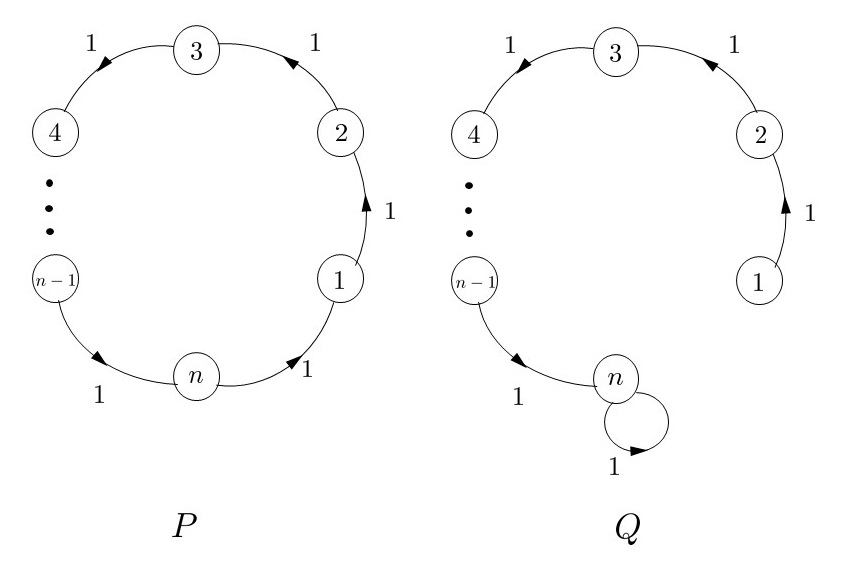
\includegraphics[scale=0.40]{diagrams/example2.jpg}
%	\caption{Example 2.}
%	\label{fig:example2}
%\end{figure}
%\end{example}
%
%\begin{example}
%\label{example:stationary_testing}
%Non symmetric MC: small difference between $P$ and $Q$ ($\dist{\word{P}{\ell}}{\word{Q}{\ell}}$ is small), but stationary distributions $\vect{p}_0$ and $\vect{q}_0$
%are vastly different. $Q$ - a ring with an edge $e=(v_1v_2)$ is removed, $v_1$ has a self-loop instead; $P$ - a similar ring with a loop, but $e$ is not removed but has a lighter
%weight of $\frac{1}{\sqrt{n}}$, while self-loop at $v_1$ has a weight of $1-\frac{1}{\sqrt{n}}$. Stationary distributions: $\vect{q}_0=\trans{(1,0,\cdots,0)}$ and
%$\vect{p}_0=\trans{(\frac{\sqrt{n}}{n+\sqrt{n}-1},\frac{1}{n+\sqrt{n}-1},\dots,\frac{1}{n+\sqrt{n}-1})}$, while $\specr{\srprod{P}{Q}}=\sqrt{1-\frac{1}{\sqrt{n}}}$.   
%%\begin{figure}[H]
%	%\centering
%		%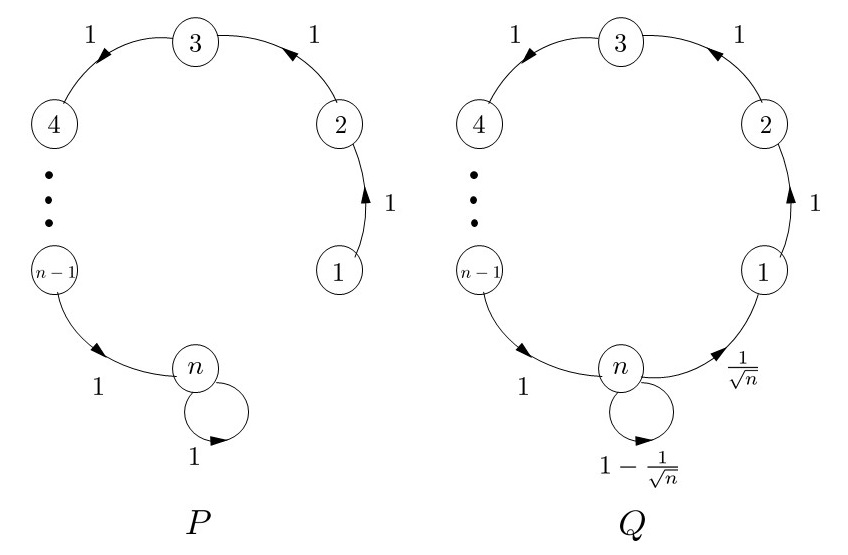
\includegraphics[scale=0.40]{diagrams/example3.jpg}
%	%\caption{Example 3.}
%	%\label{fig:example3}
%%\end{figure}
%
%\end{example}
%\begin{example}
%\label{example:same_stationary_large_dist}
%Non symmetric MC: same stationary (Uniform) distribution, $\dist{P}{Q}=1$, at average it takes $\Omega(n)$ steps to distinguish whether $P=Q$, or not.
%Two oriented cycles, 
%\[
%P\eqdef s_1\to s_2\to\cdots\to s_n\to s_1\quad\quad Q\eqdef s_1\to s_3\to s_4\cdots\to s_n\to s_2\to s_1.
%\]
%%\begin{figure}[H]
%	%\centering
%		%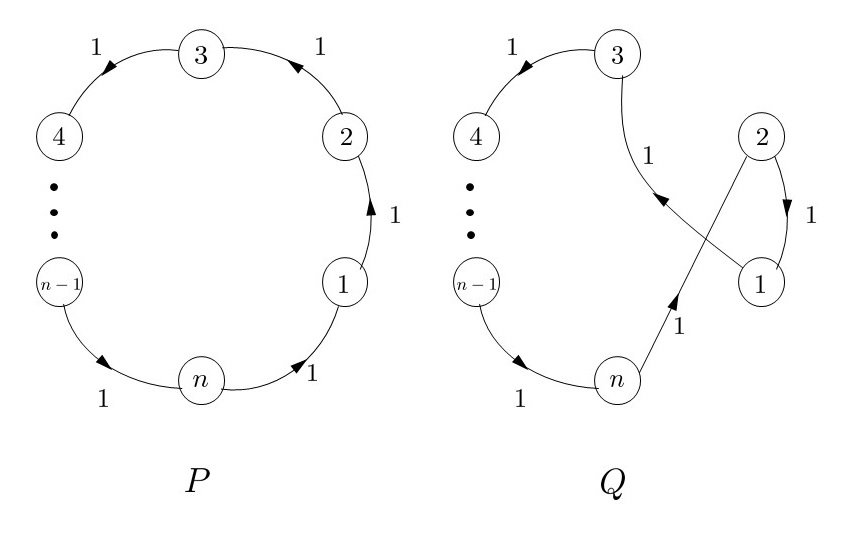
\includegraphics[scale=0.40]{diagrams/example4.jpg}
%	%\caption{Example 4.}
%	%\label{fig:example4}
%%\end{figure}
%\end{example}
%\begin{example}
%\label{example:symmetric}
%Symmetric Markov chains: $Q$ -- complete graph $Q_{ij}=1/n$; $P$ -- clique and disjoint vertex $P_{ij}=\frac{1}{n-1}, i,j\in[n-1]$, $P_{in}=P_{ni}=0, i\in[n-1],$ and 
%$P_{nn}=1$. Then $\eigi[1]=\sqrt{\frac{n-1}{n}}= 1 - \frac{1}{2n}+O(n^2)$, $\eigi[2]=\sqrt{\frac{1}{n}}$, $\eigi[3]=\cdots=\eigi[n]=0$. If Markov Chain starts from state $1$, 
%after one transition we would know almost certainly whether $w\sim P$, or $w\sim Q$. On the other hand, if $w$ starts from any other state, then it would take us about $n$ 
%observations to tell whether $w\sim P$, or $w\sim Q$. If we start from a random state, again we would need about $n$ steps to distinguish $P$ vs. $Q$.
%%\begin{figure}[H]
%	%\centering
%		%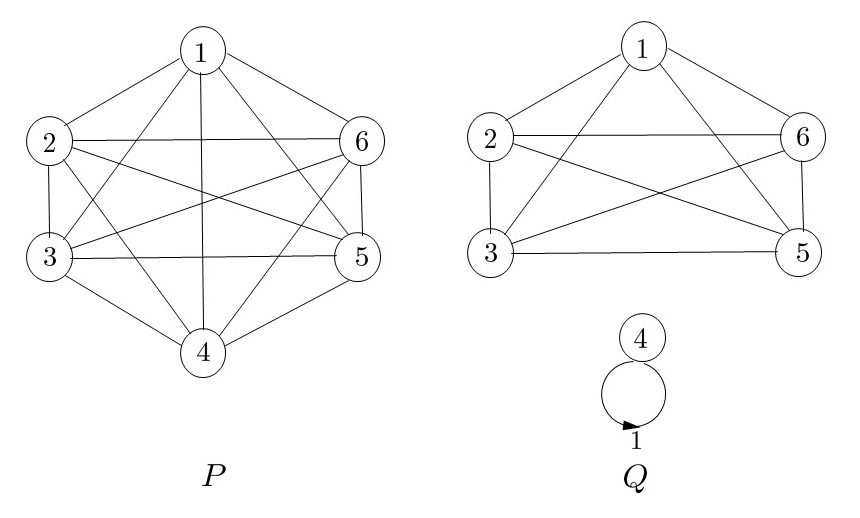
\includegraphics[scale=0.40]{diagrams/example5.jpg}
%	%\caption{Example 5.}
%	%\label{fig:example5}
%%\end{figure}
%\end{example}



\section{Identity Testing of Symmetric Markov Chains}
\label{sec:symmetric}
%Given our formal notion of distance between symmetric Markov Chains (\ref{}), we get a well defined framework (e.g. \cite{BatuFFKRW01,Paninski08,LeviRR13}) for testing properties of distributions generated by Markov Chains.
After understanding the problem of distinguishing between two given distributions, a next fundamental question is the identity testing problem where the goal is to test whether an unknown distribution $p$ from which we see a stream of samples, coincides with a given hypothesis distribution $q$. 
In this section, we study identity testing of symmetric Markov chains and provide an efficient algorithm (Theorem~\ref{th:symmetric_ub}).  
%and information theoretic lower bounds (Theorem~\ref{thm:symm-lower-bound}). 
%\nishanth{More intro needed?}
%\corrected{In this section, we present our algorithm for testing identity of symmetric Markov chains. The precise problem definition is stated below:}
We begin by giving below a formal statement of the problem:\\
%\begin{description}
%\item[Input:] $\eps$; symmetric transition matrix $Q$; stream of $m$ consecutive samples from symmetric Markov Chain $P$.
%\item[Output:] $P=Q$, or $P\neq Q$ if $1-\specr{\srprod{P}{Q}}>\eps$. 
%\end{description}
%\noindent \textbf{Identity Testing of Markov Chains:}


\begin{algorithm}[H]
%\caption{Identity Testing for Symmetric Markov Chains}
	\label{def:mc-id-testing}
\KwIn{$\eps > 0$; explicit description of a symmetric Markov chain $Q$; a trajectory $s_1\cdots s_m$ of length $m$ from a symmetric Markov Chain $P$.}
\KwOut{$P=Q$, or $P\neq Q$ if $1-\specr{\srprod{P}{Q}}>\eps$.}
\end{algorithm}



\paragraph{Our approach.}
Identity testing problem with i.i.d. samples, is a well studied problem in the
distribution testing literature. The problem is quite non trivial\footnote{It is studied by a number of works. For instance, see~\cite{BatuFFKRW01,Paninski08,ValiantV14,AcharyaDK15,DiakonikolasK16} (This is not an exhaustive list).} 
and to achieve tight sample complexity one needs to do careful estimations of collisions in observed samples.
Markov chain identity testing appears to be at least as hard as the i.i.d. identity testing problem with the added complication of dependent samples.
To avoid involved analysis of collisions among dependent samples we will instead try to find a black-box reduction of the MC testing problem to identity testing with i.i.d. samples.
%Our idea is to exploit insights about symmetric Markov chains which will allow us to reduce to the classical problem of identity testing with i.i.d. samples.
A naive attempt at such a reduction proceeds by waiting for a period of mixing time $\mixt{Q}$ of the known Markov Chain $Q$ to get one (potential) i.i.d. sample from the 
stationary distribution of $P$ (in case $P$ has mixed). If the empirical distribution for the number of visits is far from the uniform distribution, we can 
immediately reject $P$ (since if $P=Q$, then $P$ is a symmetric chain and will have the uniform distribution as the stationary) and if it is not, then we would have attained multiple transitions from a sizeable set of nodes and one could hope they contain sufficient signal to distinguish $P$ from $Q$. 
It is non-trivial to extract this signal as the mere fact that we have seen multiple samples from a single node within a short length of the trajectory introduces dependencies in our samples. That is, two samples from the same node are not independent samples from the transition distribution of that node, if it took only a little time to return to this node. Moreover, this attempt, if it works, will incur a \emph{multiplicative loss} of $\mixt{Q}$ in the sample complexity.\\
%

\noindent We take a more subtle and involved approach to achieve a successful reduction to the classical setting with i.i.d. samples. Moreover, our reduction yields an algorithm that suffers only an {\em additive loss} of $\wO{\hitt{Q}\cdot\log\left(\hitt{Q}\right)}$ in sample complexity. We reduce the Markov chain problem to the classical identity testing problem with respect to squared Hellinger distance of distributions supported on a domain of size $n^2$. Our result is always as good as the naive approach. Indeed, for symmetric chains, the hitting time cannot be larger than mixing time by more than a $c.n$ factor (where $c$ is a constant), but usually it is much smaller (in fact hitting time can be even smaller than mixing time).  
We note that many broad classes of graphs and Markov chains have close to linear hitting times, e.g., expanders, $d$-dimensional grids (which are not expanders). Below we describe how we map samples from a Markov chain to i.i.d. samples from the appropriate distribution.\\
%\nishanth{Many commonly studied Markov chains have poly(n) hitting times and hence our tester is efficient.} Below we describe at a high-level our approach.\\

\noindent \textbf{A Mapping From Infinite Words.} Consider a mapping $\infmap{\vect{k}}$ from words of infinite length $w \in W_M^{\infty}$ of an irreducible Markov chain $M$ on the state space $[n]$ to $\prod_{i=1}^{n}
[n]^{k_i}$, where $\vect{k}=(k_1,\cdots,k_n)$ is a vector of $n$ non negative integers, as follows. For each infinite word $w=s_1s_2\cdots$ and each state 
$i\in[n]$ we look at the first $k_i$ visits to state $i$ (i.e., at times $t=t_1,\dots,t_{k_i}$ with $s_{t}=i$) and write down the corresponding 
transitions in $w$, i.e., $s_{t+1}$. We note that every state is visited almost surely in $w$, since $M$ is an irreducible finite-state Markov chain. 
Therefore, mapping $\infmap{\vect{k}}$ defines a probability distribution on $\prod_{i=1}^{n}[n]^{k_i}$. Now, crucially, this distribution is independent across all different states and/or independent for a particular state $i$ because of the Markov property of Markov chains. Furthermore, a specific transition from a copy of the state $i$ is distributed according to the $i$-th row of the transition matrix $M$.

In Lemma~\ref{lem:large_deviation_bound}, we show that even for a finite length trajectory with length $ m=\widetilde{O}\left(\hitt{Q}\log\left(\hitt{Q}\right)\right. \allowbreak +\left. \frac{n}{\eps}\right)$ \footnote{in this paper, $\widetilde{O}$ always hides poly $\log(n/\eps)$ factors, but not $\hitt{Q}$.} and 
$k_i=O(\Ex{\text{\# visits to } i})=O(\frac{m}{n})$ the mapping $\infmap{\vect{k}}$ is well defined for all 
but a small fraction (in probability) of the words from the distribution $\word{M}{m}$. This effectively allows us, with high probability, to generate a large number of independent samples from the following distribution supported over $[n]\times[n]$: pick uniformly at random a state $i\in[n]$ and then observe a transition from $i$ according to transition probabilities of row $P_i$.
Indeed, to this end, we first simulate $m'=\Theta\left(\frac{m}{\log^2 (n/\eps)}\right)$ i.i.d. samples from $[n]$. These samples describe how many visits an independent sampler would make to state $i \in [n]$. Let 
$\vect{k}$ be the histogram of these $m'$ samples (note that $\max_{i} k_i \le O(m'\log n /n)$ with high probability). 
We apply $\infmap{\vect{k}}$ mapping to our stream of $m$ consecutive samples of Markov chain $P$, which is well defined with high probability. 
Apart from some small probability events ($\max_{i} k_i$ is too large, or $\infmap{\vect{k}}$ is not defined for our choice of $m$) we obtain the desired $m'$ i.i.d. 
samples. 
%Large deviation bound
\begin{lemma}
	Given an irreducible Markov chain $M$ and the mapping from infinite words $\word{M}{\infty}$ described above, for $m=\wO{\log\left(\hitt{Q}\right)\hitt{Q}}$, then 
	$\Prx{\exists~\text{state}~i~\text{s.t.}~|\{t: i=s_t\in w\}|<\frac{m}{8e\cdot n}}\le\frac{\eps^2}{n}$ where the probability is over the sampling of $\vect{k}$ and word $w$. 
%If the number of steps $m=\wO{\log\left(\hitt{Q}\right)\hitt{Q}}$, then
%\[
%\Prx{\exists \text{ state }i: |\{t: i=s_t\in w\}|<\frac{m}{8e\cdot n}}\le\frac{\eps^2}{n}.
%\] 
\label{lem:large_deviation_bound}
\end{lemma}
The proof is deferred to Appendix~\ref{app:proofs_symm}.


In the following we present our algorithm for Markov Chain identity testing and provide an upper bound on its sampling complexity.

\begin{algorithm}[H]
\caption{Independent Edges Sampler.}
\label{alg:symmetric_MC}
\SetKwData{Histogram}{Histogram}\SetKwData{Samples}{Samples}\SetKwFunction{IdentityTest}{IdentityTestIID}
\SetKwFunction{Uniform}{Uniform}
%\KwIn{$\eps$; explicit symmetric Markov chain $Q$; $m$ consecutive samples $s_1\cdots s_m$ from a symmetric Markov Chain $P$.}
%\KwOut{$P=Q$, or $P\neq Q$ if $1-\specr{\srprod{P}{Q}}>\eps$.}
\BlankLine
$\vect{k}~\leftarrow$ \Histogram ($\Theta\left(\frac{m}{\log^2 (n/\eps)}\right)$ i.i.d. \Uniform[n] samples) \;
\For{$t\leftarrow 1$ \KwTo $m-1$}{
\lIf{$|\Samples[s_t]|<\vect{k}[s_t]$}{Add $(s_t\to s_{t+1})$ to $\Samples[s_t]$}
}
\eIf{$\exists i, \text{ s.t., } |\Samples[i]|<\vect{k}[i]$}{
\KwRet \textsc{Reject};
}
{
$\Samples\leftarrow\Samples[1]\cup\dots\cup\Samples[n]$\;
\KwRet \IdentityTest($\eps,$ $\{q_{ij}=\frac{1}{n}\cdot Q_{ij}\}_{i,j\in[n]}$, \Samples)\;
}
\end{algorithm}

Algorithm~\ref{alg:symmetric_MC} uses as a black-box the tester of Algorithm 1 of~\cite{DaskalakisKW17}. The following Lemma follows from Theorem 1 of~\cite{DaskalakisKW17}. %We state the sample complexity of this result here.
\begin{lemma}
\label{lem:hellinger_idtest}
Given a discrete distribution $q$ supported on $[n]$ and access to i.i.d. samples from a discrete distribution $p$ on the same support, there is a tester which can distinguish whether $p=q$ or $\hellinger{p}{q} \ge \eps$ with probability $\ge 2/3$ using $\Ocomplex{\frac{\sqrt{n}}{\eps^2}}$ samples.
\end{lemma}
As a corollary of Lemma~\ref{lem:hellinger_idtest}, we get a test that can distinguish whether $P=Q$, or $\hellingersq{\frac{1}{n}P}{\frac{1}{n}Q}\ge\eps$ using $m=\Ocomplex{\frac{n}{\eps}}$ i.i.d samples from $\frac{1}{n}P$, which can be viewed as a distribution on a support of size $n^2$. Lemma~\ref{lem:rho_l1_distances} shows that the required distance condition for the i.i.d. sampler is implied by our input guarantee. % (proof is deferred to Appendix~\ref{app:proofs_symm}).

\begin{lemma}
	Consider two symmetric Markov chains $P$ and $Q$ on a finite state space $[n]$. Denote by $\frac{1}{n}P$ the distribution over $n^2$ elements obtained by scaling down every entry of the transition matrix $P$ by a factor $1/n$. We have,
\begin{align}
\frac{1}{2}\sum\limits_{i,j\in[n]}\left(\sqrt{\frac{P_{ij}}{n}}-\sqrt{\frac{Q_{ij}}{n}}\right)^2=
\hellingersq{\frac{1}{n}P}{\frac{1}{n}Q}\ge\dist{P}{Q}\eqdef 1-\specr{\srprod{P}{Q}} .
\end{align}
\label{lem:rho_l1_distances}
\end{lemma}
The proof of Lemma~\ref{lem:rho_l1_distances} is given in Appendix~\ref{app:proofs_symm}.

Finally, the following Theorem~\ref{th:symmetric_ub} gives an upper bound on sampling complexity of Algorithm~\ref{alg:symmetric_MC}.
We note that $\wO{\hitt{Q}}$ samples are necessary for a reduction approach to work. Indeed, if we are to simulate
$n \log n$ i.i.d. samples ($v\to u$, where $v\sim \Uniform[n]$ and $u\sim P_v$), then we shall see all states
$v\in [n]$ at least once with high probability. I.e., the random walk must visit all the states, which would require at the very least 
$\hitt{Q}$ steps in the random walk. On the other hand, our bound of $\wO{\hitt{Q}\cdot\log\left(\hitt{Q}\right)+\frac{n}{\eps}}$ is always better than a naive
bound of $\mixt{Q}\cdot\frac{n}{\eps}$, since $\hitt{Q}< n\cdot\mixt{Q}$ and, in fact, for most of the reasonable MC $\hitt{Q}$ is much less than that.

%\begin{lemma}
%$\frac{1}{n}\onenorm{P-Q}\ge 2\eps.$
%\label{lem:rho_l1_distances}
%\end{lemma}
%\begin{proof}
%We note that, as $P$ and $Q$ are symmetric matrices, so is $\srprod{P}{Q}$. Thus we have
%\be
%\label{eq:sv_def}
%1-\eps = \specr{\srprod{P}{Q}} = \max_{\twonorm{\vev}=1} \vev\circ\srprod{P}{Q}\circ\vevt.
%\ee
%If we use a particular $\vev=\frac{1}{\sqrt{n}}\onev$ in \eqref{eq:sv_def}, then we get the following inequality.
%\begin{align*}
%1-\eps \ge & \frac{1}{\sqrt{n}}\onev\circ\srprod{P}{Q}\circ\frac{1}{\sqrt{n}}\onevt = \frac{1}{n}\sum\limits_{i,j} \sqrt{P_{ij}\cdot Q_{ij}}\\
       %=  &\frac{1}{2n}\sum\limits_{i,j}\left(P_{ij}+Q_{ij}\right)-\frac{1}{2n}\sum\limits_{i,j}\left(P_{ij}+Q_{ij}-2\sqrt{P_{ij}\cdot Q_{ij}}\right)\\
        %= & 1 - \frac{1}{2n}\sum\limits_{i,j}\left(\sqrt{P_{ij}}-\sqrt{Q_{ij}}\right)^2 \ge 
        %1 - \frac{1}{2n}\sum\limits_{i,j}\left|\sqrt{P_{ij}}-\sqrt{Q_{ij}}\right|\cdot\left|\sqrt{P_{ij}}+\sqrt{Q_{ij}}\right|\\
        %= & 1 - \frac{1}{2n}\sum\limits_{i,j}\left|P_{ij}-Q_{ij}\right|=1 - \frac{1}{2n}\onenorm{P-Q}.
%\end{align*}
%Therefore, we conclude that $\frac{1}{n}\onenorm{P-Q}\ge 2\eps.$
%\end{proof}

\begin{theorem}
Given the description of a symmetric Markov chain $Q$ and access to a single trajectory of length $m$ from another symmetric Markov chain $P$,
Algorithm~\ref{alg:symmetric_MC} distinguishes between the cases $P = Q$ versus $1-\specr{\srprod{P}{Q}}>\eps$ with probability at least $2/3$, for  $m=\wO{\hitt{Q}\cdot\log\left(\hitt{Q}\right)+\frac{n}{\eps}}$. 
\label{th:symmetric_ub}
\end{theorem}
\begin{proof}
	In the case $P=Q$, the probability that Algorithm~\ref{alg:symmetric_MC} proceeds to IID tester, i.e., it
	does not reject $P$, because of small number of visits to a state, is at least
	$\Prx{\forall i\in[n]~|\{t: i=s_t\in w\}|>\frac{m}{8e\cdot n}}\cdot\Prx{\forall i: \frac{m}{8e\cdot n}>k_i} \ge 
	\left(1-\frac{\eps^2}{n}\right)\cdot\left(1-\frac{\eps^2}{n}\right)\ge 1-\frac{2\eps^2}{n}$. In the previous estimate, we used Lemma~\ref{lem:large_deviation_bound} 
	to bound $\Prx{\forall i\in[n]~|\{t: s_t\in w, s_t=i\}|>\frac{m}{8e\cdot n}}$, the fact that $\Prx{\frac{m}{8e\cdot n} \le k_i} \le \frac{\eps^2}{n^2}$ (follows from a Chernoff bound), and a union bound.  IID tester then correctly accepts $P=Q$ with probability at least $4/5$.
	Hence, the error probability is at most $1/5+\frac{2\eps^2}{n}<1/3$.
	
	For the case $P\neq Q$, Lemma~\ref{lem:rho_l1_distances} says that if $1-\specr{\srprod{P}{Q}}>\eps$, then distributions passed down to the IID tester 
	$\{p: p_{ij}=\frac{1}{n}P_{ij}\}$ and $\{q: q_{ij}=\frac{1}{n}Q_{ij}\}$ are at least $\eps$ far in Hellinger-squared distance. A black-box application of Lemma \ref{lem:hellinger_idtest} implies a  $\Ocomplex{\frac{n}{\eps}}$ sampling complexity for the IID tester in our case.
	Furthermore,
	random mapping $\infmap{\vect{k}}:\word{P}{\infty}\to p$ (where $\vect{k}$ is a histogram of $m'=\Theta\left(\frac{m}{\log^2 (n/\eps)}\right)$ i.i.d. uniform samples from $[n]$) produces
	$m'$ i.i.d. samples from $p$. Hence, if Algorithm~\ref{alg:symmetric_MC} has sufficient samples from $P$ to define the mapping $\infmap{\vect{k}}$, it would be able to distinguish $p$ and $q$ with probability
	at least $2/3$. On the other hand, if Algorithm~\ref{alg:symmetric_MC} gets finite number of samples which are not sufficient to define the mapping $\infmap{\vect{k}}$, then 
	it correctly rejects $P$ before even running the IID tester.
	
	Thus in both cases the probability of error is at most $1/3$.
\end{proof}


%Our approach:
%\begin{enumerate}
%\item We define a mapping $\infmap{\vect{k}}$ from infinite words $\word{M}{\infty}$ of an irreducible Markov chain $M$ to $\prod_{i=1}^{n}
%[n]^{k_i}$, where $\vect{k}=(k_1,\cdots,k_n)$ is a vector of $n$ positive integers, as follows. For each infinite word $w=s_1s_2\cdots$ and each state 
%$i\in[n]$ we look at the first $k_i$ visits to state $i$ (i.e., at times $t=t_1,\dots,t_{k_i}$ with $s_{t}=i$) and write down the corresponding 
%transitions in the infinite word $w$, i.e., $s_{t+1}$. We note that every state is visited almost surely in $w$, since $M$ is an irreducible Markov chain. 
%Therefore, mapping $\infmap{\vect{k}}$ defines a probability distribution on $\prod_{i=1}^{n}[n]^{k_i}$. We note that by construction the realized values 
%in $\prod_{i=1}^{n}[n]^{k_i}$ of each fixed state $i$ and across all different 
%states are independent.
%\item We show that for large enough $m=\wO{\covert{M}+n\cdot f(\eps)}$ and 
%$k_i=\frac{\Ex{\text{\# visits to } i}}{\log^2 n}=\frac{m}{n\log^2 n}$ the mapping
%$\infmap{\vect{k}}$ is well defined for a finite $m$ number of samples for all but a small fraction of the words in $\word{M}{\infty}$. (Here we use 
%the fact that $M$ is symmetric irreducible MC, implying that $\onev$ is the stationary distribution.)
%\item We are going to use as a black-box \cite{AcharyaDK15} for identity $L_1$-testing with i.i.d. samples from a distribution with a support of size $n^2$. We want to simulate a number of i.i.d samples where we first pick uniformly at random a state $i\in[n]$ and then observe  
%transition from $i$ according to transition probabilities of $P$. We first simulate $m'$ (to be determined later) i.i.d. samples from $[n]$. Let 
%$\vect{k}$ be the histogram of these $m'$ samples (note that $\max_{i} k_i \le O(m'\log n /n)$ with high probability). 
%We apply $\infmap{\vect{k}}$ mapping to our stream of $m$ consecutive samples of Markov chain $P$, which is well defined with high probability. 
%Apart from a small fraction of events (when $\max_{i} k_i$ is too large, or $\infmap{\vect{k}}$ is not defined) we obtain the desired $m'$ i.i.d. 
%samples. 
%
%Now \cite{AcharyaDK15} says that we can test using $m=\Ocomplex{\frac{n}{\eps^2}}$ samples whether $P=Q$, or tell that $P\neq Q$, if $\frac{1}{n}\onenorm{P-Q}\ge\eps$. We use our $m'=\wO{\frac{n}{\eps^2}}$ samples to detect whether $\frac{1}{n}\onenorm{P-Q}\ge\eps$. It remains to show that the latter guarantee is implied by our notion of distance.
%
%We note that, as $P$ and $Q$ are symmetric matrices, so is $\srprod{P}{Q}$. Thus we have
%\be
%\label{eq:sv_def}
%1-\eps = \specr{\srprod{P}{Q}} = \max_{\twonorm{\vev}=1} \vev\circ\srprod{P}{Q}\circ\vevt.
%\ee
%
%If we use a particular $\vev=\frac{1}{\sqrt{n}}\onev$ in \eqref{eq:sv_def}, then we get the following inequality.
%\begin{align*}
%1-\eps \ge & \frac{1}{\sqrt{n}}\onev\circ\srprod{P}{Q}\circ\frac{1}{\sqrt{n}}\onevt = \frac{1}{n}\sum\limits_{i,j} \sqrt{P_{ij}\cdot Q_{ij}}\\
       %=  &\frac{1}{2n}\sum\limits_{i,j}\left(P_{ij}+Q_{ij}\right)-\frac{1}{2n}\sum\limits_{i,j}\left(P_{ij}+Q_{ij}-2\sqrt{P_{ij}\cdot Q_{ij}}\right)\\
        %= & 1 - \frac{1}{2n}\sum\limits_{i,j}\left(\sqrt{P_{ij}}-\sqrt{Q_{ij}}\right)^2 \ge 
        %1 - \frac{1}{2n}\sum\limits_{i,j}\left|\sqrt{P_{ij}}-\sqrt{Q_{ij}}\right|\cdot\left|\sqrt{P_{ij}}+\sqrt{Q_{ij}}\right|\\
        %= & 1 - \frac{1}{2n}\sum\limits_{i,j}\left|P_{ij}-Q_{ij}\right|=1 - \frac{1}{2n}\onenorm{P-Q}.
%\end{align*}
%
%Therefore, we conclude that $\frac{1}{n}\onenorm{P-Q}\ge 2\eps.$
%
%\end{enumerate}
%\input{tight_upper_bound}

\section{A Lower Bound for Identity Testing of Symmetric Markov Chains}
\label{sec:symmetric_lb}

\label{sec:symm-lower-bound}
In this section we provide an information theoretic lower bound to the identity testing problem on Markov chains defined in Section~\ref{sec:symmetric}. 
%will show that any algorithm that tests identity of a symmetric Markov chain requires a word of length $\Omega\left({\frac{n}{\eps}}\right)$ from the Markov chain. 
%where $n$ is the number of states in the Markov chain.
%We will use Le Cam's two point method to show our lower bound.
\begin{theorem}
\label{thm:symm-lower-bound}
There exists a constant $c > 0$ and an instance of the identity testing problem for symmetric Markov chains such that any tester on this instance requires
a word of length at least $c\frac{n}{\eps}$ as input to produce the correct output with probability $> 0.99$. %(\ref{def:mc-id-testing})
%There is an instance of the identity testing problem for symmetric Markov chain $Q$ on $n$ states 
%that requires a word of length at least $\Omega(\frac{n}{\eps})$ from $P$ to distinguish between cases 
%$P=Q$ vs. $1-\specr{\srprod{P}{Q}} \ge \eps$  with probability at least $\frac{99}{100}$, for $\eps=\omega(n^{-1/3})$.
%
%There exists a constant $c>0$,such that any algorithm which is given the description of a symmetric Markov chain $Q$ and 
%sample access to words from a symmetric Markov chain $P$ on $n$ states, and distinguishes between the cases $P \equiv Q$ 
%and $1-\specr{\srprod{P}{Q}} \ge \eps$ with probability at least $99/100$ requires at least $k \geq \frac{cn}{\eps}$ samples.
\end{theorem}
The full proof of Theorem~\ref{thm:symm-lower-bound} is given in Appendix~\ref{app:sec_symm_lb}. The high level idea is to construct a Markov chain $Q$ and a family of chains $\mathcal{P}$ such that it is hard to distinguish $Q$ from a randomly chosen $\bar{P} \in \mathcal{P}$ by only looking at trajectories of length $o(n/\eps)$. The chain $Q$ and the family $\mathcal{P}$ we work with are described below (we think of symmetric Markov chains as weighted undirected graphs with multi-edges allowed).
\begin{description}
	\item[Markov Chain $Q$:] complete double graph on $n$ vertices with uniform weights, i.e., 
	\[
	\forall \quad i\neq j \quad\quad (ij)_1, (ij)_2\in E  \quad\quad  Q_{(ij)_1}=Q_{(ij)_2}=\frac{1}{2(n-1)}.
	%Q_{(ij)_1}=\frac{1}{2(n-1)} \quad\quad Q_{(ij)_2}=\frac{1}{2(n-1)}\quad\quad \text{ for any } i\neq j.
	\]
	\item[Family $\mathcal{P}$:] for any pair of vertices $i\neq j$ there are two bidirectional edges $(ij)_1$, $(ij)_2$
	with weights randomly (and independently for each pair of $(i,j)$) chosen to be either
	\[
	P_{(ij)_1}, P_{(ij)_2}=\frac{1\pm \sqrt{8\eps}}{2(n-1)},
	\quad\quad\text{ or }\quad\quad
	P_{(ij)_1},P_{(ij)_2}=\frac{1\mp \sqrt{8\eps}}{2(n-1)}.
	\]
	%\[
	%\begin{cases}
	%P_{(ij)_1}&=\frac{1+4\sqrt{\eps}}{2n-2}, \\
	%P_{(ij)_2}&=\frac{1-4\sqrt{\eps}}{2n-2}
	%\end{cases}
	%\text{ or }
	%\begin{cases}
	%P_{(ij)_1}&=\frac{1-4\sqrt{\eps}}{2n-2}, \\
	%P_{(ij)_2}&=\frac{1+4\sqrt{\eps}}{2n-2}
	%\end{cases}  
	%\]
	%
	%
	%for every state $i$, bidirectional transition probabilities to states $j$ and $j'$, for each $j > i$, 
	%are randomly chosen to be either $\frac{1+4\sqrt{\eps}}{2n-2},\frac{1-4\sqrt{\eps}}{2n-2}$ or 
	%$\frac{1-4\sqrt{\eps}}{2n-2},\frac{1+4\sqrt{\eps}}{2n-2}$ respectively. The family consists of every 
	%Markov chain which can be generated by this process.
	%for every state $i$, bidirectional transition probabilities to states $j$ and $j'$, for each $j > i$, 
	%are randomly chosen to be either $\frac{1+4\sqrt{\eps}}{2n-2},\frac{1-4\sqrt{\eps}}{2n-2}$ or 
	%$\frac{1-4\sqrt{\eps}}{2n-2},\frac{1+4\sqrt{\eps}}{2n-2}$ respectively. The family consists of every 
	%Markov chain which can be generated by this process.
\end{description}
From the construction above it is clear that one needs to observe a number of collisions to distinguish $Q$ from a randomly chosen member of $\mathcal{P}$. The proof proceeds by a careful analysis of these collision probabilities to bound the TV distance between words of length $k$ from $Q$ and from a randomly chosen $\bar{P} \in \mathcal{P}$.



\section{Open Questions}
\label{sec:open}
In this paper, we proposed a new framework for studying property testing questions on Markov chains. 
There seem to be multiple avenues for future research and abundant number of open problems arising from this framework. 
We first list some questions which may be of interest here.
\begin{enumerate}
\item What is the optimal sample complexity for identity testing on symmetric Markov chains? In this paper, we show an upper bound of $\wO{\hitt{Q}\cdot\log\left(\hitt{Q}\right)+\frac{n}{\eps}}$ samples (Theorem \ref{th:symmetric_ub}). We conjecture that $\Theta\left( \frac{n}{\eps}\right)$ (same as our lower bound) is the right sample complexity for this problem and an explicit dependence on the hitting time of chain $Q$ may not be necessary. It is implicitly captured to an extent by the guarantee we get from the parameter $\eps$.
%\item What is the optimal sample complexity for identity testing on the sparse Markov chains defined in Section~\ref{sec:shuffle}? In this paper, we show an upper bound of $\widetilde{O}\left( \frac{n^{3/2}}{\epsilon^2} \right)$ (Theorem \ref{th:sparse_ub}). We conjecture that $\Theta\left( \frac{n}{\eps^2}\right)$ (same as our lower bound) is the right sample complexity for this problem.

\item As there is a natural operation of taking a convex combination of Markov chains, it is natural to ask how our spectral definition of distance 
$1-\specr{\srprod{P}{Q}}$ between two symmetric chains changes if we substitute either $P$ or $Q$ with a convex combination of $P$ and $Q$. How does the distance now relate to the original value?
%\item How is the difference parameter $\eps=1-\specr{\srprod{P}{Q}}$ between two Markov chains $P$ and $Q$ related to the difference between Markov chains $P^k$ and $Q^k$,i.e., states in Markov chains $P$ and $Q$ being observed only at intervals of size $k$? 
\item Given $\eps_2 \ge \eps_1$, and access to words from each of two chains, can we distinguish whether the two chains are $\le \eps_1$-close or $\ge \eps_2$-far? This problem, known as two-sample testing in literature, is another interesting direction using our framework.
\end{enumerate}
%More broadly, we are interested in the following research directions
%\begin{enumerate}
%\item Testing other properties of Markov chains, e.g., testing closeness of two Markov chains.
%\item Testing Hidden Markov Models.
%\end{enumerate}


%\nishanth{
%Reminders:
%\begin{enumerate}
%\item Do we want to change the title of the paper so as to sell the framework? Although we solve testing problems only, what we have is quite general and can be applied to statistical problems other than testing as well for e.g. learning). 
%
%%\item Add remark saying that we considered other seemingly more natural and simpler distance notion and mention why they don't capture the behavior well. For example, for GSR L1 between the parameter vectors isn't a good distance notion as it gives large weight to parameters which are of little significance.
%\end{enumerate}
%}


%\bibliographystyle{alpha}
\bibliography{bib}

\appendix
\section{Examples}
\label{app:sec_examples}
\begin{figure}[H]
	\centering
	%\begin{subfigure}[b]
		%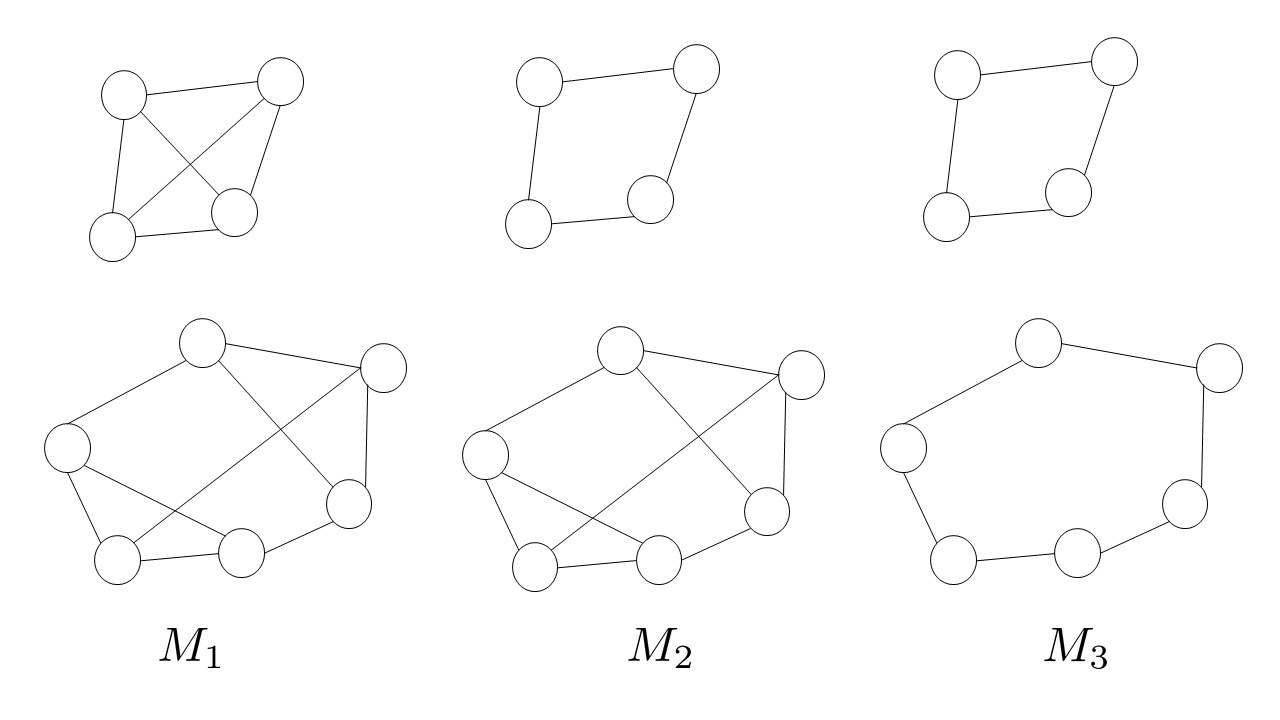
\includegraphics[scale=0.16]{diagrams/example1.jpg}
		%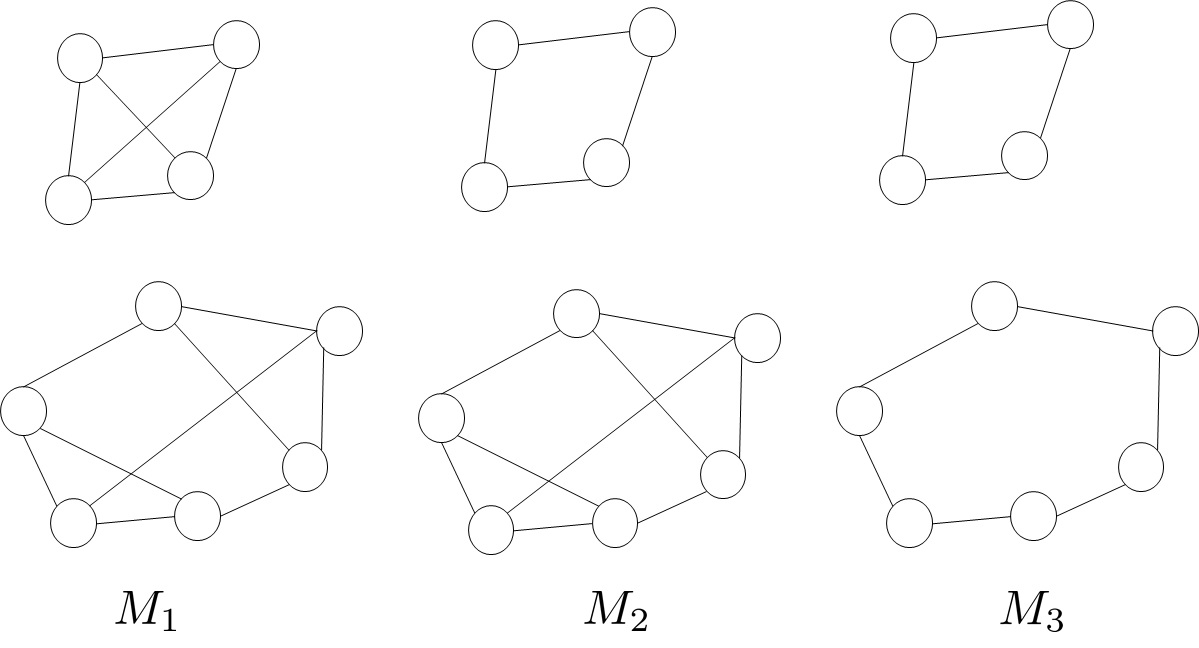
\includegraphics[width=\textwidth]{diagrams/Example_1.png}
		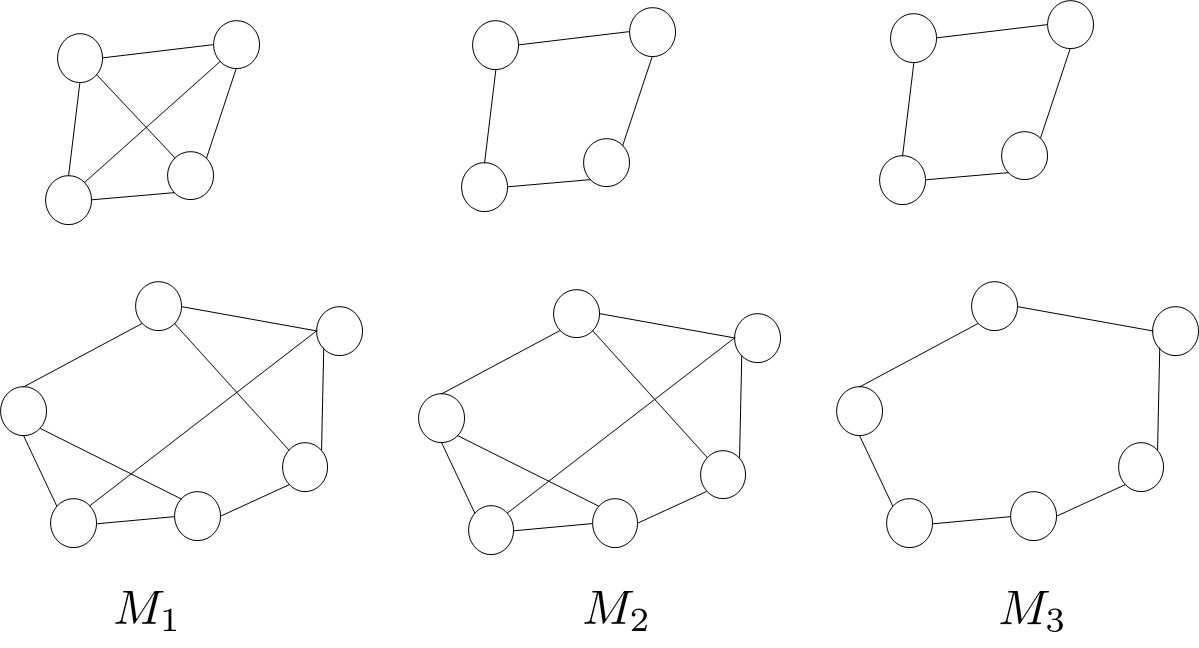
\includegraphics[width=0.7\textwidth]{Ex1.png}
		\caption{$\dist{M_1}{M_2}=1-\specr{\srprod{M_1}{M_2}}$ is not a metric. $\dist{M_1}{M_2}=\dist{M_2}{M_3}=0,$ but 
			$\dist{M_1}{M_3}> 0$.}
		\vspace{3ex}
		\label{fig:example1}
	%\end{subfigure}
	
	%\begin{subfigure}[b]{4.95cm}
		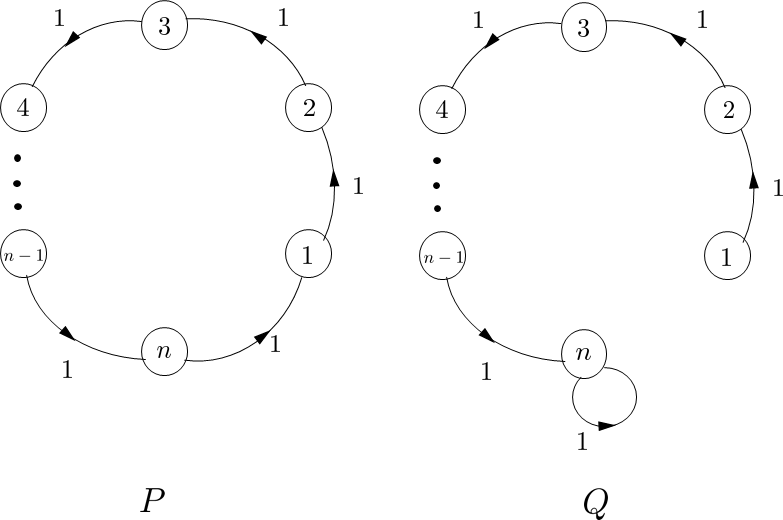
\includegraphics[width=0.5\textwidth]{Ex2.png}
		\caption{To distinguish $P$ vs. $Q$ walking from a random state we need $\Omega(n)$ steps, but $\dist{P}{Q}=1$.}
		\label{fig:example2}
	%\end{subfigure}
	\hspace{3pt}
\end{figure}

\begin{figure}[H]
\centering
	%\begin{subfigure}[b]{4.95cm}
		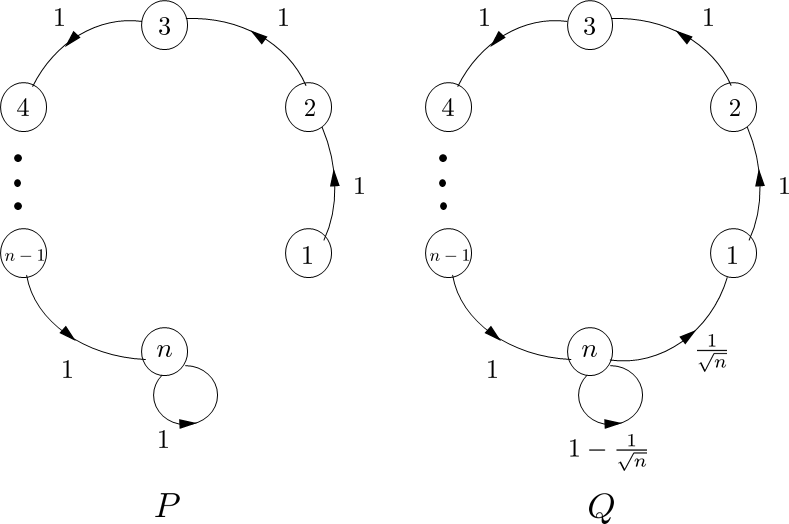
\includegraphics[width=0.5\textwidth]{Ex3.png}
		\caption{$\dist{P}{Q}=o(1)$, stationary distributions $\vect{q}_0,\vect{p}_0$ 
			are different: $\dtv{\vect{q}_0}{\vect{p}_0}=1-o(1)$.}
		\label{fig:example3}
	%\end{subfigure}
	\hspace{3pt}
	%\begin{subfigure}[b]{4.95cm}
		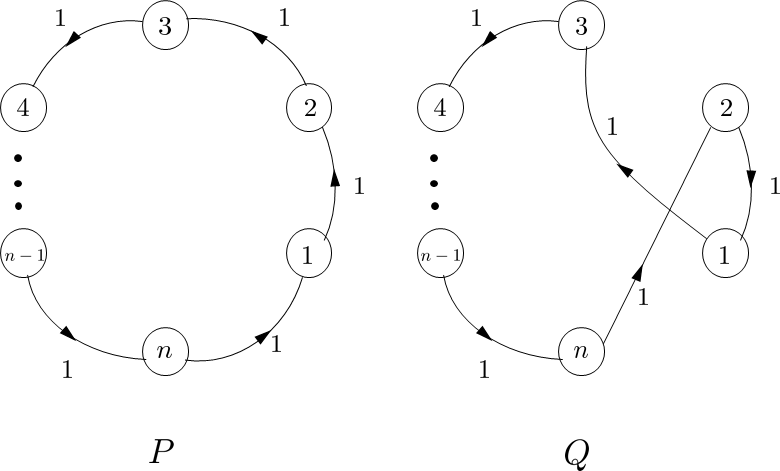
\includegraphics[width=0.5\textwidth]{Ex4.png}
		\caption{$\dist{P}{Q}=1$. Uniform is stationary	for both $P$ and $Q$. 
			On average $\Omega(n)$ steps to tell $P\neq Q$.}
		\label{fig:example4}
	%\end{subfigure}
	
	\hspace{5pt}	
	%\begin{subfigure}[b]{7cm}
		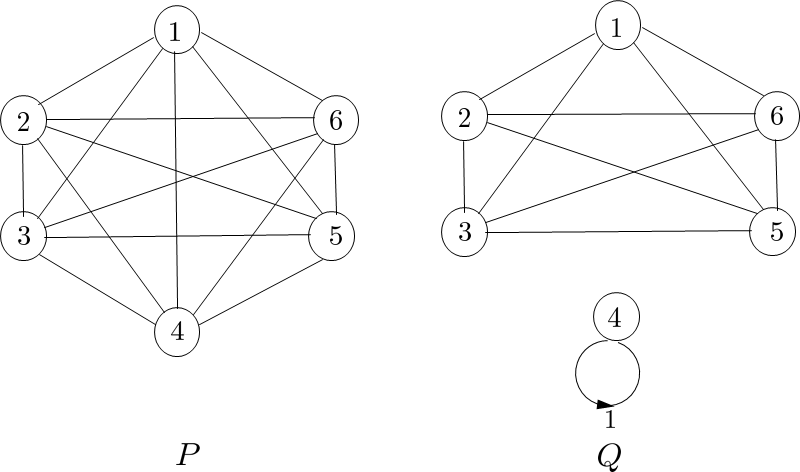
\includegraphics[width=0.7\textwidth]{Ex5.png}
		\caption{After one step from state $4$, we would know if $w\sim P$, or $w\sim Q$. 
			If $w$ starts from any other state $s_0\neq 4$, it would take many steps.}
		\vspace{3ex}
		\label{fig:example5}
	%\end{subfigure}
\end{figure}
	
	
	\vspace{5ex}
	\begin{table}
	\begin{tabular}{ | l | p{0.8\textwidth} |}
		\cline{2-2}
		%\multicolumn{1}{|c|}{Description}
		
		\multicolumn{1}{c|}{} &  \multicolumn{1}{c|}{Description} \\ \hline
		Example~\ref*{fig:example1} & Two disjoint connected components. \\ \hline
		Example~\ref*{fig:example5} & $Q$ -- clique $K_n$; $P$ -- clique $K_{n-1}$ and disjoint vertex.
		Eigenvalue of $\srprod{P}{Q}$: $\eigi[1]=\sqrt{\frac{n-1}{n}}=1-o(1)$, 
		$\eigi[2]=\sqrt{\frac{1}{n}}$, $\eigi[3]=\cdots=\eigi[n]=0$	\\  \hline												
		Example~\ref*{fig:example2} & $P$ -- oriented cycle, $Q$ -- cycle with one link substituted by a loop.\\ \hline
		Example~\ref*{fig:example3} & $P$ -- oriented cycle with edge $e=(v_1v_2)$ substituted by a loop at $v_1$; 
		$Q$ is almost like $P$, but $e$ has weight $\frac{1}{\sqrt{n}}$, loop at $v_n$ has weight $1-\frac{1}{\sqrt{n}}$. 
		Stationary distributions: $\vect{p}_0=\trans{(1,0,\cdots,0)}$ 
		and $\vect{q}_0=\trans{(\frac{\sqrt{n}}{n+\sqrt{n}-1},\frac{1}{n+\sqrt{n}-1},\dots,\frac{1}{n+\sqrt{n}-1})}$. 
		$\specr{\srprod{P}{Q}}=\sqrt{1-\frac{1}{\sqrt{n}}}$.   \\  \hline
		Example~\ref*{fig:example4} & Two oriented cycles $P\eqdef s_1\to s_2\to\cdots\to s_n\to s_1$ and 
		$Q\eqdef s_1\to s_3\to s_4\cdots\to s_n\to s_2\to s_1$.	\\  \hline											
	\end{tabular}
	\caption{Examples.} \label{fig:examples}
	\end{table}


%\begin{figure}[H]
	%\floatconts
	%\subfigure[b]{
		%%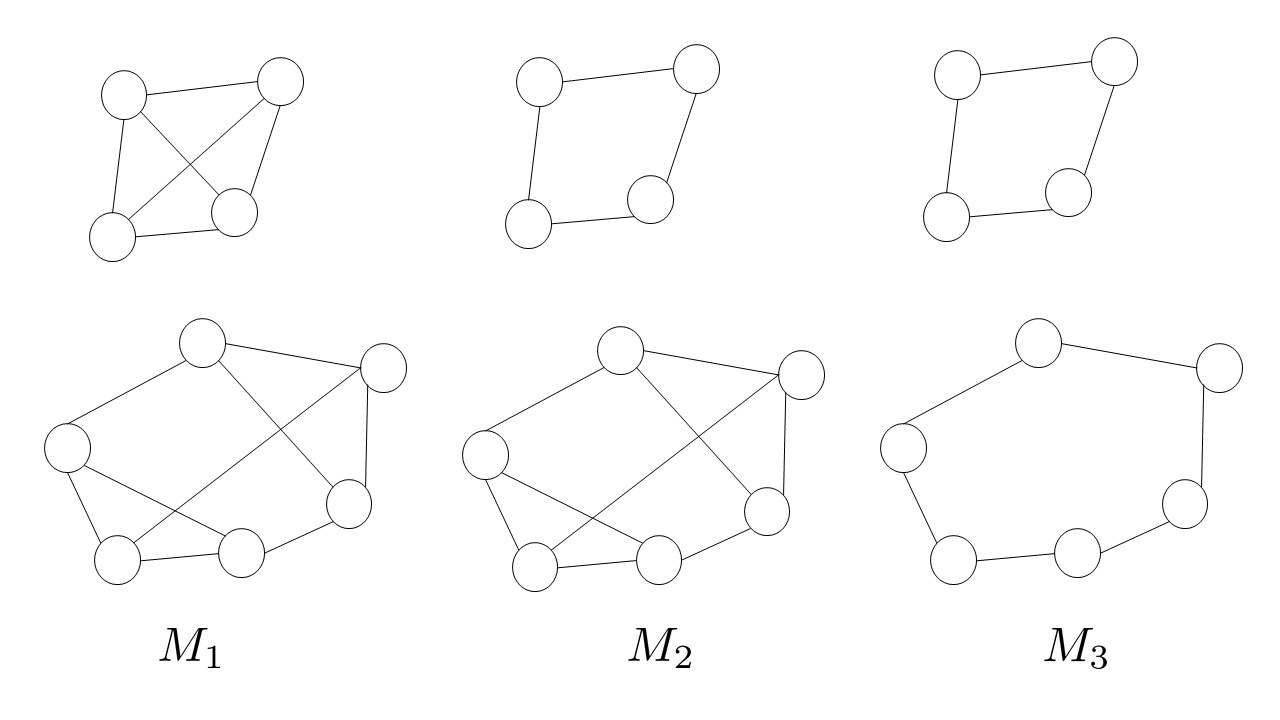
\includegraphics[scale=0.16]{diagrams/example1.jpg}
		%%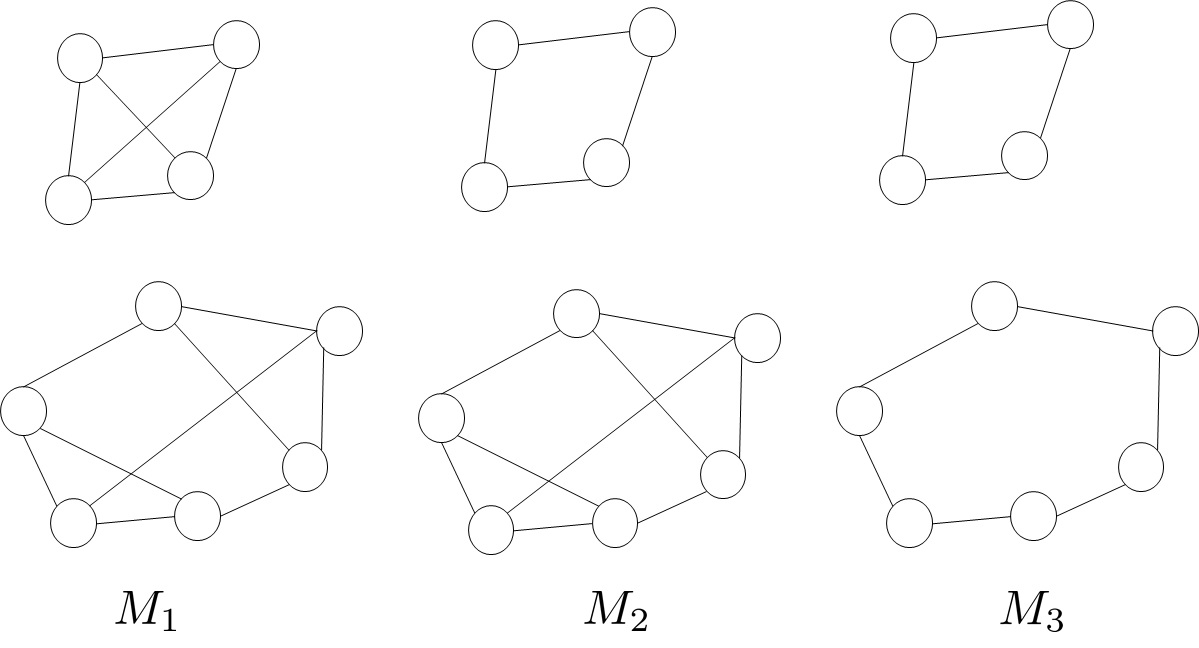
\includegraphics[width=\textwidth]{diagrams/Example_1.png}
		%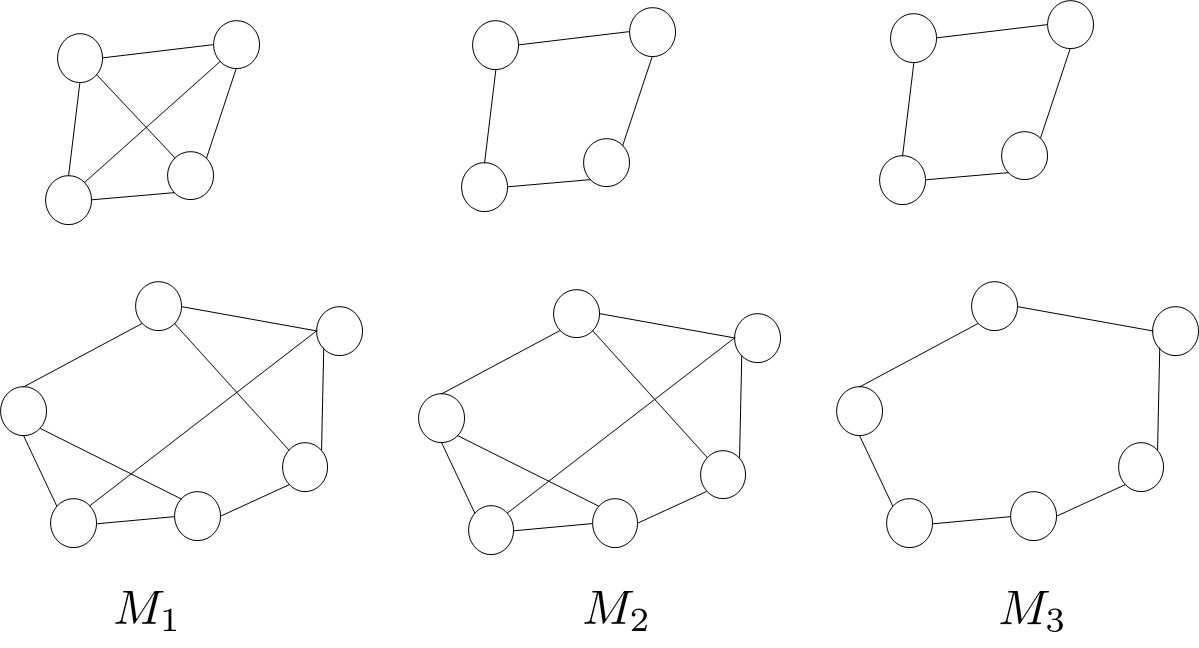
\includegraphics[width=7.45cm]{Ex1.png}
		%\caption{$\dist{M_1}{M_2}=1-\specr{\srprod{M_1}{M_2}}$ is not a metric. $\dist{M_1}{M_2}=\dist{M_2}{M_3}=0,$ but 
			%$\dist{M_1}{M_3}> 0$.}
		%\vspace{3ex}
		%\label{fig:example1}
	%}
	%%\end{subfigure}
	%\hspace{5pt}
	%\floatconts	
	%\subfigure[b]{
		%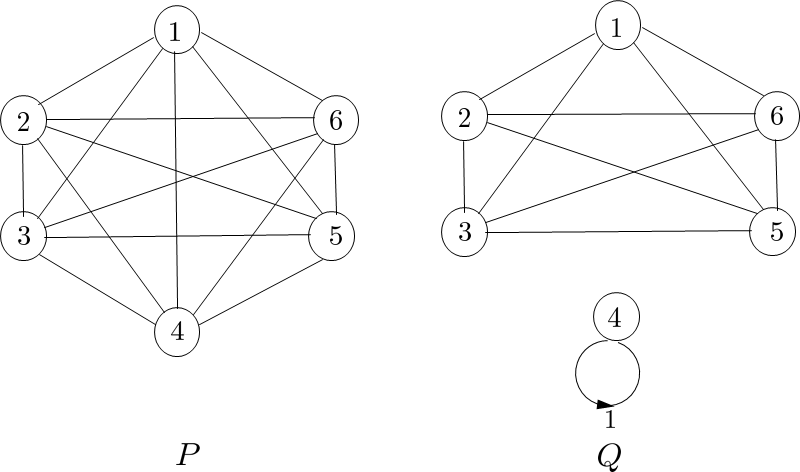
\includegraphics[width=0.45\textwidth]{Ex5.png}
		%\caption{After one step from state $4$, we would know if $w\sim P$, or $w\sim Q$. 
			%If $w$ starts from any other state $s_0\neq 4$, it would take many steps.}
		%\vspace{3ex}
		%\label{fig:example5}
	%}
	%%\end{subfigure}
	%\floatconts
	%\subfigure[b]{
		%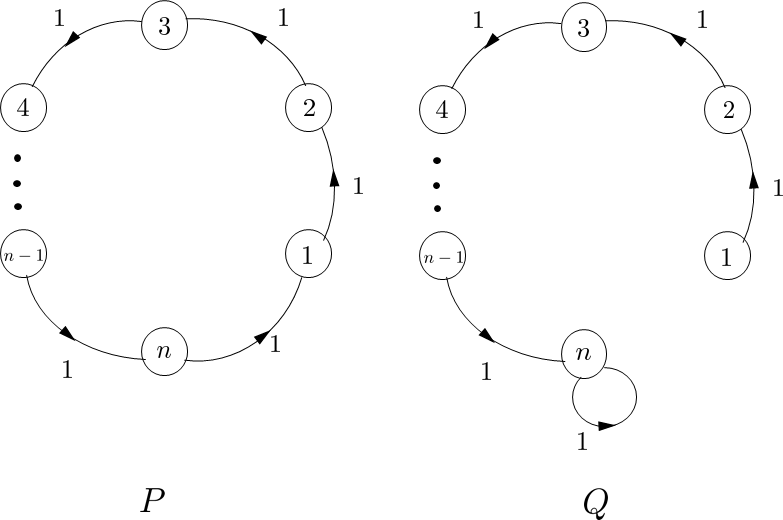
\includegraphics[width=0.9\textwidth]{Ex2.png}
		%\caption{To distinguish $P$ vs. $Q$ walking from a random state we need $\Omega(n)$ steps, but $\dist{P}{Q}=1$.}
		%\label{fig:example2}
	%}
	%%\end{subfigure}
	%\hspace{3pt}
	%\floatconts	
	%\subfigure[b]{
		%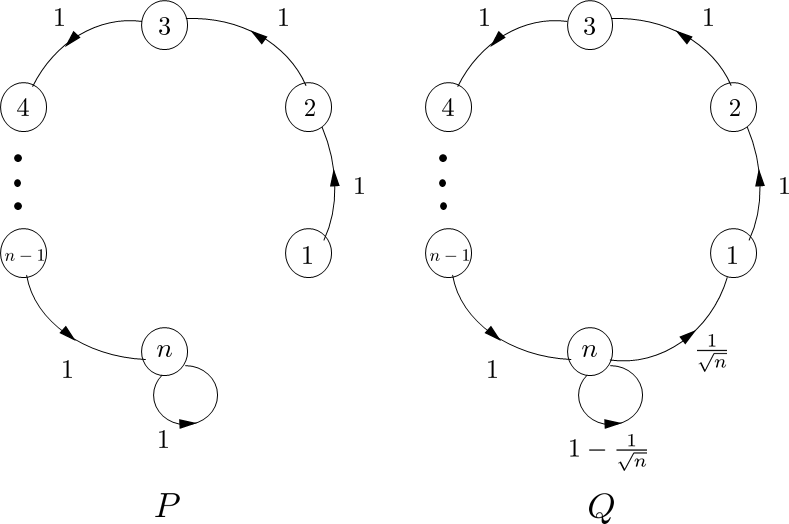
\includegraphics[width=0.9\textwidth]{Ex3.png}
		%\caption{$\dist{P}{Q}=o(1)$, stationary distributions $\vect{q}_0,\vect{p}_0$ 
			%are different: $\dtv{\vect{q}_0}{\vect{p}_0}=1-o(1)$.}
		%\label{fig:example3}
	%}
	%%\end{subfigure}
	%\hspace{3pt}
	%\floatconts
	%\subfigure[b]{
		%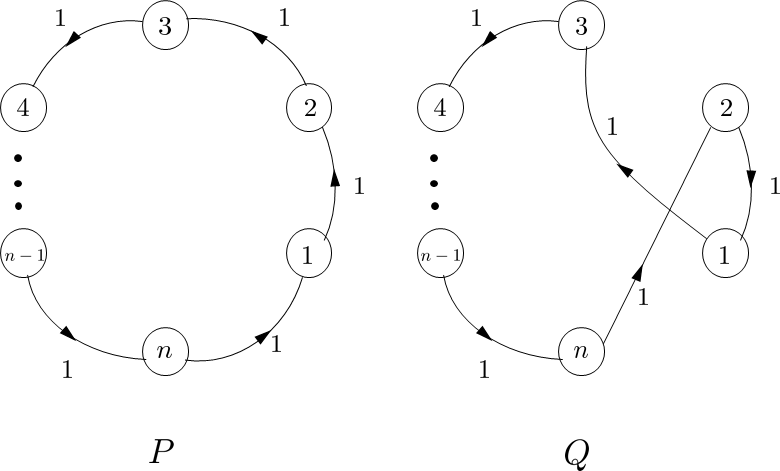
\includegraphics[width=0.9\textwidth]{Ex4.png}
		%\caption{$\dist{P}{Q}=1$. Uniform is stationary	for both $P$ and $Q$. 
			%On average $\Omega(n)$ steps to tell $P\neq Q$.}
		%\label{fig:example4}
	%}
	%%\end{subfigure}
	%
	%\vspace{5ex}
	%\begin{tabular}{ | l | p{0.8\textwidth} |}
		%\cline{2-2}
		%%\multicolumn{1}{|c|}{Description}
		%
		%\multicolumn{1}{c|}{} &  \multicolumn{1}{c|}{Description} \\ \hline
		%Example~\ref*{fig:example1} & Two disjoint connected components. \\ \hline
		%Example~\ref*{fig:example5} & $Q$ -- clique $K_n$; $P$ -- clique $K_{n-1}$ and disjoint vertex.
		%Eigenvalue of $\srprod{P}{Q}$: $\eigi[1]=\sqrt{\frac{n-1}{n}}=1-o(1)$, 
		%$\eigi[2]=\sqrt{\frac{1}{n}}$, $\eigi[3]=\cdots=\eigi[n]=0$	\\  \hline												
		%Example~\ref*{fig:example2} & $P$ -- oriented cycle, $Q$ -- cycle with one link substituted by a loop.\\ \hline
		%Example~\ref*{fig:example3} & $P$ -- oriented cycle with edge $e=(v_1v_2)$ substituted by a loop at $v_1$; 
		%$Q$ is almost like $P$, but $e$ has weight $\frac{1}{\sqrt{n}}$, loop at $v_n$ has weight $1-\frac{1}{\sqrt{n}}$. 
		%Stationary distributions: $\vect{p}_0=\trans{(1,0,\cdots,0)}$ 
		%and $\vect{q}_0=\trans{(\frac{\sqrt{n}}{n+\sqrt{n}-1},\frac{1}{n+\sqrt{n}-1},\dots,\frac{1}{n+\sqrt{n}-1})}$. 
		%$\specr{\srprod{P}{Q}}=\sqrt{1-\frac{1}{\sqrt{n}}}$.   \\  \hline
		%Example~\ref*{fig:example4} & Two oriented cycles $P\eqdef s_1\to s_2\to\cdots\to s_n\to s_1$ and 
		%$Q\eqdef s_1\to s_3\to s_4\cdots\to s_n\to s_2\to s_1$.	\\  \hline											
	%\end{tabular}
	%
	%\caption{Examples.} \label{fig:examples}
%\end{figure}

\section{Missing proofs from Section~\ref{sec:distance}}
\label{app:proofs_dist}
%\begin{lemma}[\cite{Kazakos78}] %\label{lemma:kazakos lemma}
%Suppose $P$ and $Q$ are Markov Chains over states $[n]$, $\vect{p}$ and $\vect{q}$ are probability distributions of the initial state. Let $\word{P}{\ell}$, $\word{Q}{\ell}$ 
%be the distributions denoting a length $\ell$ trajectory of Markov Chains $P$ (resp. $Q$) starting at a random node $s_0$ sampled from $\vec{p}$ (resp. $\vec{q}$). Moreover, define 
%the vector $\srprod{\vect{p}}{\vect{q}}\eqdef\left[\sqrt{p_s\cdot q_s}\right]_{s\in[n]}$ and the matrix $\srprod{P}{Q}\eqdef\left[\sqrt{P_{ij}\cdot Q_{ij}}~ \right]_{i,j\in[n\times n]}$. Then:
%\be
%%\label{eq:hellinger_square_algebraic}
%1-\hellingersq{\word{P}{\ell}}{\word{Q}{\ell}}=\srprodt{\vect{p}}{\vect{q}}\circ \left(\srprod{P}{Q}\right)^{\ell} \circ \onev,
%\ee
%\end{lemma}
\begin{prevproof}{Lemma}{lemma:kazakos lemma}
	\begin{multline*}
	1-\hellingersq{\word{P}{\ell}}{\word{Q}{\ell}}=\sum_{w=s_0\ldots s_\ell}\sqrt{\Prlong[P]{w}\Prlong[Q]{w}}
	=\trans{\left[\sum_{\substack{w=s_0\ldots s_{\ell}\\s_\ell=s}}\sqrt{\Prlong[P]{w}\Prlong[Q]{w}}\right]}_{s\in[n]}\circ\onev\\
	=\trans{\left[\sum_{r\in[n]}\sqrt{\Prlong[P]{r\to s}\Prlong[Q]{r\to s}}\sum_{\substack{w=s_0\ldots s_{\ell-1}\\s_{\ell-1}=r}}\sqrt{\Prlong[P]{w}\Prlong[Q]{w}}\right]}_{s\in[n]}\circ\onev\\
	=\trans{\left[\sum_{\substack{w=s_0\ldots s_{\ell-1}\\s_{\ell-1}=r}}\sqrt{\Prlong[P]{w}\Prlong[Q]{w}}\right]}_{r\in[n]}\circ
	\begin{bmatrix}
	&\vdots&\\
	\cdots&\sqrt{P_{rs}\cdot Q_{rs}}&\cdots\\
	&\vdots&
	\end{bmatrix}_{r,s\in[n\times n]}
	\circ\onev
	\\
	=\trans{\left[\sum_{\substack{w=s_0\ldots s_{\ell-1}\\s_{\ell-1}=r}}\sqrt{\Prlong[P]{w}\Prlong[Q]{w}}\right]}_{r\in[n]}\circ\srprod{P}{Q}\circ\onev
	=\srprodt{\vect{p}}{\vect{q}}\circ \left(\srprod{P}{Q}\right)^{\ell} \circ \onev,
	%\label{eq:hellinger_square_algebraic}
	\end{multline*}
\end{prevproof}


\begin{prevproof}{Claim}{cl:eigval_less_than_one}
	Note that $\frac{P+Q}{2}$ is a stochastic matrix that 
	entry-wise dominates matrix $\srprod{P}{Q}$ with non-negative entries. Therefore,
	$
	\eigi[1]\cdot\scalprod{\eigvli[1]}{\onev}=\eigvlit[1]\circ\srprod{P}{Q}\circ\onev\le\eigvlit[1]\circ\left[\frac{P+Q}{2}\right]\circ\onev
	=\eigvlit[1]\circ\onev=\scalprod{\eigvli[1]}{\onev},
	$
	where $\onev$ is vector with all $1$ entries. We get $\eigi[1]\le 1$, since $\scalprod{\eigvli[1]}{\onev}>0$.
	
	For the case of equality, if $P$ and $Q$ have the same essential communicating class $C$, then matrix $\srprod{P}{Q}$ has the same transition 
	probabilities as Markov chains $P$ and $Q$ restricted to the vertices of $C$. We note that $C$ is a stochastic 
	matrix and, therefore, its largest positive eigenvalue is one. Hence, $\specr{\srprod{P}{Q}}\ge\specr{C} = 1.$
	
	If $\specr{\srprod{P}{Q}}=1$, we apply Perron-Frobinius theorem to $\srprod{P}{Q}$ to get  
	that the largest eigenvalue $\eigi[1]=\specr{\srprod{P}{Q}}=1$ has corresponding (left) eigenvector $\eigvli[1]$ with non-negative entries. 
	We observe that $\eigvlit[1]\circ\left(\frac{P+Q}{2}-\srprod{P}{Q}\right)\circ\onev=0$, 
	and all entries of the matrix in this expression are non-negative. This implies that $P_{ij}=Q_{ij}$ for every strictly positive coordinates 
	$i$ of the eigenvector $\eigvli[1]$ and any $j\in[n]$. Since $\eigvlit[1]\circ\srprod{P}{Q}=\eigvlit[1]$, we also have $P_{ij}=Q_{ij}=0$ for any positive 
	coordinate $i$ and zero coordinate $j$ of eigenvector $\eigvli[1]$. Therefore, the set of vertices corresponding to positive coordinates of $\eigvli[1]$ 
	form a component (which might have more than one connected component of $P$ and $Q$) such that $P=Q$ on these vertices.  
\end{prevproof}


\begin{prevproof}{Claim}{cl:symm_spectrum}
	We first consider the average-case model for the starting state. Note that $\srprod{P}{Q}$ is a symmetric matrix. 
	Let $\eigvi[1],\dots,\eigvi[n]$ be normalized orthogonal eigenvectors of $\srprod{P}{Q}$, corresponding to 
	real $\eigi[1]\ge\dots\ge\eigi[n]$ eigenvalues. Then for RHS of \eqref{eq:forall_states_eigenvalue} we have
	\be
	\frac{1}{n}\onevt\circ \left(\srprod{P}{Q}\right)^{\ell}\circ\onev=\frac{1}{n}\onevt\circ\left(\sum_{i=1}^n\eigi\cdot\eigvi\circ\eigvit\right)^\ell\circ\onev
	=\sum_{i=1}^n\eigi^\ell\cdot\frac{1}{n}\iprod{\onev}{\eigvi}^2=(*)
	\label{eq:definition_star}
	\ee
	Now we can write an upper and lower bound on $(*)$ in terms of $\eigi[1]^\ell$ (assuming that $\ell$ is even):
	\begin{multline*}
	\frac{\eigi[1]^\ell}{n}=\frac{\eigi[1]^\ell}{n}\twonorm{\eigvi[1]}^2\le\eigi[1]^\ell\cdot\frac{1}{n}\onenorm{\eigvi[1]}^2
	\le(*) \le
	\sum_{i=1}^n\eigi^\ell\cdot\frac{1}{n}\onenorm{\eigvi}^2\le\sum_{i=1}^n\eigi^\ell\cdot\twonorm{\eigvi}^2=\sum_{i=1}^n\eigi^\ell\le n\cdot\eigi[1]^\ell,  
	\end{multline*}
	where in the second inequality we used Perron-Frobenius theorem stating that all coordinates of $\eigvi[1]$ are non negative. 
	Consequently, these bounds imply that $\ell=\Theta\left(\frac{1}{\eps}\right)$ up to a $\log n$ factor, if $\specr{\srprod{P}{Q}}=\eigi[1]=1-\eps$. 
	I.e., $\ell=\wTheta{\frac{1}{\eps}}$.
	
	For the worst-case assumption on the starting state, it is sufficient to show an upper bound $\ell=\Ocomplex{\frac{\log n}{\eps}}$. 
	In this case~\eqref{eq:definition_star} becomes
	\[
	\onevti\circ \left(\srprod{P}{Q}\right)^{\ell}\circ\onev=\sum_{i=1}^n\eigi^\ell\cdot\iprod{\onevi}{\eigvi}\cdot\iprod{\onev}{\eigvi}
	\le\sum_{i=1}^n|\eigi|^\ell\cdot\infnorm{\eigvi}\cdot\onenorm{\eigvi}
	\le\sum_{i=1}^n|\eigi|^\ell\cdot \sqrt{n}\le n^{1.5}\cdot\eigi[1]^\ell,
	\]
	since $\onenorm{\eigvi}\le\sqrt{n}\twonorm{\eigvi}=\sqrt{n}$, and $\infnorm{\eigvi}\le\twonorm{\eigvi}=1$.
\end{prevproof}




\section{Missing proofs from Section~\ref{sec:symmetric}}
\label{app:proofs_symm}
\iffalse
\begin{lemma}
	\label{lem:hitting-vs-mixing}
	For a symmetric Markov chain $M$ on a discrete state space of size $n$, 
	$$\hitt{M} \le \mixt{M}n.$$
\end{lemma}
\begin{proof}
	
\end{proof}
\fi


\begin{prevproof}{Lemma}{lem:large_deviation_bound}
%\begin{proof}
	To simplify notations we denote by $\Delta\eqdef 2\hitt{Q}$. By union bound over all states $i$ it is enough to show that $\Prx{|\{t: i=s_t\in w\}|<\frac{m}{8e\cdot n}}\le\frac{\eps^2}{n^2}$ 
	for each fixed state $i$. We can make sure that in the first $\frac{m}{2}$ steps state $i$ is visited at least once with probability 
	at least $1-\frac{\eps^2}{n^3}$. Once we visited state $i$, instead of hitting time for state $i$ we can analyze the {\em return time} $\returnt$ for $i$.
	Note that for symmetric Markov chains $\frac{1}{n}\onev$ (uniform distribution) is a stationary distribution. Therefore, every state appears at average once 
	in every $n$ steps in an infinite word from $\word{Q}{\infty}$. In other terms, the expectation of $\returnt$ for each 
	state $i$ is exactly $n$. By definition of hitting time we have that in $\frac{\Delta}{2}$ steps the probability 
	of reaching a particular state $i$ from any other state $j$ is greater than $1-1/e$ (or any other given constant). It implies that $\Prx{\returnt \ge \frac{\Delta}{2}\cdot C}\le e^{-C}$
	for any $C\in\N$. Indeed, one can show this by induction on parameter $C$. 
	Notice that if the random walk did not return to $i$ after $C-1$ steps it has stopped at some state $j\neq i$. Then for any choice of $j$ by definition of the hitting time 
	the random walk will return to $i$ with probability at least $1/e$ in the next $\frac{\Delta}{2}$ steps. It is not hard to get a similar bound $\Prx{\returnt \ge \Delta\cdot C}\le e^{-C}$ for any $C\ge 1, C\in\R$. To simplify notations we use $X$ to denote the random variable $\returnt$ 
	and $X_1,\dots,X_\ell$ to denote $\ell$ i.i.d. samples of $X$. We have  
	
	\be
	X\ge 0\quad\text{and}\quad\forall C\in\R_{\ge 1},\Prx{X \ge \Delta\cdot C}\le e^{-C} \quad\text{and}\quad \Ex{X}=n.
	\label{eq:ineq_return}
	\ee
	
	We only need to show that $\Prx{X_1+\cdots+X_\ell > m/2} \le \frac{\eps^2}{n^2}$ for $\ell=\frac{m}{8e\cdot n}$.
	To this end, we use a standard technique for large deviations and apply Markov's inequality to the moment generating function of $X_1 + \cdots + X_\ell$,
	
	%\begin{multline*}
	\be
	\Prx{X_1+\cdots+X_\ell > m/2}=\Prx{e^{\theta\cdot(X_1+\cdots+X_\ell)} > e^{\theta\cdot m/2}}\le\frac{\Ex{e^{\theta\cdot(X_1+\cdots+X_\ell)}}}{e^{\theta\cdot m/2}} \\
	=\frac{\Ex{e^{\theta X}}^\ell}{e^{\theta\cdot m/2}}
	\label{eq:MGF_markov}
	\ee
	%\end{multline*}
	We note that given restrictions \eqref{eq:ineq_return} on $X$ maximum of $\Ex{e^{\theta X}}$ for any fixed $\theta>0$ is attained at 
	\[
	X^*\sim
	\begin{cases}
	\Delta\cdot x  & x\in[C_0,\infty) \text{ with probability density function } e^{-x}\\
	0 & \text{with remaining probability }1-e^{-C_0},
	\end{cases}
	\]
	where constant $C_0>1$ is such that $\Ex{X^*}=n$. Indeed, distribution $X^*$ maximizes \eqref{eq:MGF_markov} due to simple variational inequality:
	$\epsilon\cdot e^{\theta\cdot a}+\epsilon\cdot e^{\theta\cdot b}<\epsilon\cdot e^{\theta\cdot (a-c)}+\epsilon\cdot e^{\theta\cdot (b+c)}$ for any $b \ge a \ge c > 0$, and probability mass $\epsilon>0$.
	This inequality allows us to increase $\Ex{e^{\theta\cdot X}}$ and not change $\Ex{X}$ by tweaking density function $f(x)$ of $X$ 
	$f'(a-c)=f(a-c)+\epsilon$, $f'(a)=f(a)-\epsilon$, $f'(b)=f(b)-\epsilon,$ $f'(b+c)=f'(b+c)+\epsilon$, ($f'(x)=f(x)$ for all other $x$), for some $c\le a$. 
	The only time we cannot apply this incremental change is when $X=X^*$.
	
	We have 
	\be
	\label{eq:C0}
	\Ex{X^*}=\Delta(C_0+1)e^{-C_0} = n.
	\ee 
	We set $\theta\eqdef\frac{1}{2\Delta\log\Delta}$ in \eqref{eq:MGF_markov}. Now we are ready to estimate $\Ex{e^{\theta\cdot X}}$.
	To simplify notations we denote $\gamma\eqdef\frac{1}{2\log\Delta}$.
	\begin{multline}
	\Ex{e^{\theta\cdot X}}=1-e^{-C_0}+\int_{C_0}^{\infty}e^{\theta\cdot\Delta\cdot x}\cdot e^{-x}\,\mathrm{d}x=
	1-e^{-C_0}+\int_{C_0}^{\infty}e^{-x\cdot(1-\frac{1}{2\log\Delta})}\,\mathrm{d}x\\
	=1-e^{-C_0}+\frac{e^{-C_0(1-\gamma)}}{1-\gamma}=1+e^{-C_0}\left(\frac{e^{C_0\gamma}}{1-\gamma}-1\right).
	\label{eq:expectation_MGF}
	\end{multline}
	We notice that $\gamma C_0<1$, since from \eqref{eq:C0} we can conclude that $\frac{e^{C_0}}{C_0+1}=\frac{\Delta}{n}\implies C_0<2\log\Delta=1/\gamma$. The last implication can be obtained as follows: for $C_0 > 2.52,$ we have $C_0 - \frac{C_0}{2}\le C_0-\ln(1+C_0)=\ln(\frac{\Delta}{n})$. Now, we can estimate $e^{\gamma C_0}\le 1 + e\cdot\gamma C_0$ in \eqref{eq:expectation_MGF}. Furthermore, since $\gamma<1/2$ we have
	the term $\frac{e^{C_0\gamma}}{1-\gamma}-1$ in \eqref{eq:expectation_MGF} to be at most $2e\gamma(C_0+1)$. With this estimate we continue \eqref{eq:expectation_MGF}
	\be
	\Ex{e^{\theta\cdot X}}\le 1+e^{-C_0}2e\gamma(C_0+1)=1+\frac{e\cdot n}{\Delta\log\Delta}.
	\label{eq:expectation_MGF2}
	\ee
	We apply estimate~\eqref{eq:expectation_MGF2} and formula $\theta=\frac{1}{2\Delta\log\Delta}$ to~\eqref{eq:MGF_markov} to obtain
	\[
	\Prx{X_1+\cdots+X_\ell > m/2}\le \frac{\left(1+\frac{e\cdot n}{\Delta\log\Delta}\right)^\ell}{e^{m/4\Delta\log\Delta}}
	\le\frac{e^{m/8\Delta\log\Delta}}{e^{m/4\Delta\log\Delta}}=e^{\frac{-m}{8\Delta\log\Delta}}<\frac{\eps^2}{n^2},
	\]
	where in the second inequality we used the fact $\left(1+\frac{e\cdot n}{\Delta\log\Delta}\right)^{\frac{\Delta\log\Delta}{e\cdot n}}<e$, and to get the last inequality
	we used $m=\wOm{\Delta\log\Delta}$ (where in $\widetilde{\Omega}$ the hidden dependency is only on  $\log \eps$ and $\log n$).
%\end{proof}
\end{prevproof}


%\begin{lemma}
%	Consider two symmetric Markov chains $P$ and $Q$ on a finite state space $[n]$. Denote by $\frac{1}{n}P$ the distribution over $n^2$ elements obtained by scaling down every entry of the transition matrix $P$ by a factor $1/n$. We have,
%\begin{align}
%\frac{1}{2}\sum\limits_{i,j\in[n]}\left(\sqrt{\frac{P_{ij}}{n}}-\sqrt{\frac{Q_{ij}}{n}}\right)^2=
%\hellingersq{\frac{1}{n}P}{\frac{1}{n}Q}\ge\eps.
%\end{align}
%%\label{lem:rho_l1_distances}
%\end{lemma}
\begin{prevproof}{Lemma}{lem:rho_l1_distances}
	%\begin{proof}
	We note that, as $P$ and $Q$ are symmetric matrices, so is $\srprod{P}{Q}$. Thus we have
	\be
	\label{eq:sv_def}
	1-\eps = \specr{\srprod{P}{Q}} = \max_{\twonorm{\vev}=1} \vevt\circ\srprod{P}{Q}\circ\vev.
	\ee
	If we use a particular $\vev=\frac{1}{\sqrt{n}}\onev$ in \eqref{eq:sv_def}, then we get the following inequality.
	\begin{align*}
	1-\eps \ge & \frac{1}{\sqrt{n}}\onevt\circ\srprod{P}{Q}\circ\frac{1}{\sqrt{n}}\onev = \frac{1}{n}\sum\limits_{i,j} \sqrt{P_{ij}\cdot Q_{ij}} =  1-\hellingersq{\frac{1}{n}P}{\frac{1}{n}Q},
	\end{align*}
	which implies $\hellingersq{\frac{1}{n}P}{\frac{1}{n}Q}\ge\eps$.
\end{prevproof}



%\section{Reduction to adversarial testing}
%\input{reduction_to_advers_testing}
%\label{app:sec_red_advers_test}
%\section{Distance between two MC (missing proofs)}
%\label{app:sec_dist}
%\input{appendix_dist}
%
%\section{Identity Testing of Symmetric MC (missing proofs)}
%\label{app:sec_symmetric}
%\input{appendix_symmetric}
%
\section{Proof of the Lower Bound}
\label{app:sec_symm_lb}
%\subsubsection{The Lower Bound Proof}
Here we present the proof of Theorem~\ref{thm:symm-lower-bound}.


\begin{prevproof}{Theorem}{thm:symm-lower-bound}
We use Le Cam's two point method and construct a symmetric Markov chain $Q$ and a class of symmetric Markov chains $\mathcal{P}$ s.t.  
(i) every $P \in \mathcal{P}$ is at least $\eps$ far from $Q$ for a given constant $\eps$. That is $1-\specr{\srprod{P}{Q}} \geq \eps$ for any $P \in \mathcal{P}$;
(ii) there is a constant $c > 0$, s.t. it is impossible to distinguish a word of length $m$ generated by a randomly chosen 
Markov chain $\bar{P} \sim \mathcal{P}$, from a word of length $m$ produced by $Q$ with probability equal to or greater than $\frac{99}{100}$ for $m\le\frac{cn}{\eps}$.
To prove (ii) we show that the total variation distance between the $m$-word distributions obtained from the two processes, $Q$ and $\bar{P}$, is small when $m<\frac{cn}{\eps}$ for 
some constant $c$. We denote distribution of length $m$ words obtained from $Q$ by $\word{Q}{m}$, and from MC $\bar{P}\sim\mathcal{P}$ by $\word{\mathcal{P}}{m}$. 
%\begin{itemize}
%\item The word distribution of words of length $t$ obtained from $Q$ (represented by $\word{Q}{t}$).
%\item The word distribution of words of length $t$ obtained from a Markov chain $\bar{P}$ chosen uniformly at random from the family $\mathcal{P}$ (represented by $\word{\bar{P}}{t}$).
%\end{itemize}
We represent symmetric MC as undirected weighted graphs $G=(V,E)$. 
We allow graph to have multi-edges (this is helpful to provide an intuitive understanding of the lower bound construction and is not 
essential). We can ultimately remove all multi-edges and give a construction with only simple edges by 
doubling the number of states.

\begin{description}
	\item[Markov Chain $Q$:] complete double graph on $n$ vertices with uniform weights, i.e., 
	\[
	\forall \quad i\neq j \quad\quad (ij)_1, (ij)_2\in E  \quad\quad  Q_{(ij)_1}=Q_{(ij)_2}=\frac{1}{2(n-1)}.
	%Q_{(ij)_1}=\frac{1}{2(n-1)} \quad\quad Q_{(ij)_2}=\frac{1}{2(n-1)}\quad\quad \text{ for any } i\neq j.
	\]
	\item[Family $\mathcal{P}$:] for any pair of vertices $i\neq j$ there are two bidirectional edges $(ij)_1$, $(ij)_2$
	with weights randomly (and independently for each pair of $(i,j)$) chosen to be either
	\[
	P_{(ij)_1}, P_{(ij)_2}=\frac{1\pm \sqrt{8\eps}}{2(n-1)},
	\quad\quad\text{ or }\quad\quad
	P_{(ij)_1},P_{(ij)_2}=\frac{1\mp \sqrt{8\eps}}{2(n-1)}.
	\]
	%\[
	%\begin{cases}
	%P_{(ij)_1}&=\frac{1+4\sqrt{\eps}}{2n-2}, \\
	%P_{(ij)_2}&=\frac{1-4\sqrt{\eps}}{2n-2}
	%\end{cases}
	%\text{ or }
	%\begin{cases}
	%P_{(ij)_1}&=\frac{1-4\sqrt{\eps}}{2n-2}, \\
	%P_{(ij)_2}&=\frac{1+4\sqrt{\eps}}{2n-2}
	%\end{cases}  
	%\]
	%
	%
	%for every state $i$, bidirectional transition probabilities to states $j$ and $j'$, for each $j > i$, 
	%are randomly chosen to be either $\frac{1+4\sqrt{\eps}}{2n-2},\frac{1-4\sqrt{\eps}}{2n-2}$ or 
	%$\frac{1-4\sqrt{\eps}}{2n-2},\frac{1+4\sqrt{\eps}}{2n-2}$ respectively. The family consists of every 
	%Markov chain which can be generated by this process.
	%for every state $i$, bidirectional transition probabilities to states $j$ and $j'$, for each $j > i$, 
	%are randomly chosen to be either $\frac{1+4\sqrt{\eps}}{2n-2},\frac{1-4\sqrt{\eps}}{2n-2}$ or 
	%$\frac{1-4\sqrt{\eps}}{2n-2},\frac{1+4\sqrt{\eps}}{2n-2}$ respectively. The family consists of every 
	%Markov chain which can be generated by this process.
\end{description}
To make this instance a simple graph with at most one bidirectional edge between any pair of vertices we apply 
a standard graph theoretic transformation: we make a copy $i'$ for each vertex $i$; for each pair of double edges 
$e_1=(ij)_1, e_2=(ij)_2$ construct $4$ edges $(ij),(ij'),(i'j),(i'j')$ with weights $w(ij)=w(i'j')=w(e_1)$ and $w(ij')=w(i'j)=w(e_2)$. 
%See Appendix~\ref{app:sec_symm_lb} for complete proof.
%We complete the rest of the proof in Section \ref{app:sec_symm_lb}.
%We apply standard graph theoretic transformation to make this instance a simple graph with one bidirectional edge
%between any pair of vertices. To this end we make a copy $i'$ for each vertex $i$ and for each pair of double edges 
%$e_1=(ij)_1, e_2=(ij)_2$ construct $4$ edges $(ij),(ij'),(i'j),(i'j')$ with weights $w(ij)=w(i'j')=w(e_1)$ and $w(ij')=w(i'j)=w(e_2)$.
%In fact, we will ultimately remove this assumption and give a construction with only simple edges by 
%increasing the number of states by a factor of 2. \nishanth{intuition about construction goes here}
%All Markov chains in our lower bound construction will have the same set $S$ of states and $|S| = 2n$. Hence each 
%transition matrix is a $2n \times 2n$ square matrix whose row $i$ contains the transition probabilities from state 
%$i$ to the other states.

As all Markov chains $Q$ and $P\in\mathcal{P}$ are symmetric with respect to the starting state, we can assume without loss of generality that word $w$ starts from
the state $i=1$. First, we observe that for the simple graph $2n$-state representation  
\begin{lemma}
	\label{clm:p-far-from-q}
	Every Markov chain $P \in \mathcal{P}$ is at least $\eps$-far from $Q$.
\end{lemma}
\begin{proof}
	For any $P \in \mathcal{P}$, it can be seen that 
	$$\srprod{P}{Q}\circ \onev = \left(\frac{\sqrt{1+\sqrt{8\eps}}+\sqrt{1-\sqrt{8\eps}}}{2}\right)\cdot\onev.$$
	By Perron-Frobenius theorem $\onev$ is the unique eigenvector corresponding to the largest absolute value eigenvalue.  
	%and since all its entries are non-negative, by Perron-Frobenius theorem for non-negative matrices, we get that $\onev$ is the 
	%eigenvector corresponding to the eigenvalue with the largest absolute value. 
	Hence, $\specr{\srprod{P}{Q}} = \frac{\sqrt{1+\sqrt{8\eps}}+\sqrt{1-\sqrt{8\eps}}}{2}$ which by Taylor series expansion implies $1-\specr{\srprod{P}{Q}}\ge\eps+\frac{5}{2}\eps^2+o(\eps^2)
	\ge \eps$ for any $\eps<\frac{1}{8}$.
	%\begin{align}
	%1-\rho\left(\srprod{P}{Q} \right) &= 1-\frac{\sqrt{1+4\sqrt{\eps}}+\sqrt{1-4\sqrt{\eps}}}{2} \notag\\
	%&\geq 1-\left(\frac{1+\frac{4\sqrt{\eps}}{2}-\frac{16\eps}{8}+\frac{64\eps^{1.5}}{16}+1-\frac{4\sqrt{\eps}}{2}-\frac{16\eps}{8}+\frac{64\eps^{1.5}}{16}}{2}\right) \label{eq:bytaylor}\\
	%&\geq 2\eps - 4\eps^{1.5} \notag\\
	%&\geq \eps \label{eq:eps-small}
	%\end{align}
	%where (\ref{eq:bytaylor}) follows from Taylor's inequality and (\ref{eq:eps-small}) follows for small enough $\eps$\nishanth{technically inaccurate}.
\end{proof}

%\nishanth{Collision definition changes now due to duplication of states.}
We say that a given word $w=s_1\ldots s_m$ from a Markov chain $P$ represented as a multi-edge graph on $n$ states has a $(ij)$ {\em collision}, 
if any state transition between states $i$ and $j$ (in any direction along any of the edges $(ij)_1,(ij)_2$) occurs more than once in $w$. We now 
state and prove the following claims about the Markov chain family $\mathcal{P}$.


\begin{lemma}
	\label{clm:num-collisions}
	Consider a word $w$ of length $m$ drawn from $Q$. The expected number of collisions in $w$ is
	at most $\Ocomplex{\frac{m^2}{n^2}}=\Ocomplex{\frac{1}{\eps^2}}$. 
	%and the probability of $w$ having a collision is $\leq \frac{t^2}{2(n-1)^2}$.
\end{lemma}
\begin{prevproof}{Lemma}{clm:num-collisions}
	Let $I_w(t_1,t_2,(ij))$ indicate the event that in the multi-edge interpretation of the Markov chain $P$, the transition along $(ij)$ edge occurs at times $t_1<t_2$  in $w$. 
	%That is, $I_w(t_1,t_2,i \rightarrow j) = 1$ if $s_{t_1} = i, s_{t_1+1} = j$ and $s_{t_2} = i, s_{t_2+1} = j$. $I_w(t_1,t_2,i \rightarrow j) = 0$ otherwise. 
	First, we observe that $\Prx{s_{t_1}=s | s_{t_1-1}=x} \leq \frac{1}{n-1}$ and $\Prx{s_{t_2}=s | s_{t_1-1}=x} \leq \frac{1}{n-1}$ for all $x$ and both $s=i$ or $s=j$.
	Thus for any $t_2\ge t_1+2$ by a union bound for all four possible cases of $s_{t_1},s_{t_1+1},s_{t_2},s_{t_2+1}\in\{i,j\}$ we have 
	$$\E\left[I_w(t_1,t_2,(ij)) \right] \leq \frac{4}{(n-1)^4}.$$
	Similarly, for the case $t_2=t_1+1$ we can obtain 
	$$\E\left[I_w(t_1,t_2,(ij)) \right] \leq \frac{2}{(n-1)^3}.$$
	%$$\Prx{s_{t_1}=i} \leq \frac{1}{n-1}$$
	%when considering the worst possible distribution of state $s_1$. This is because $\Prx{s_{t_1}=s | s_{t_1-1}=x} \leq 1/(n-1)$ for all $x$. 
	%Similarly $\Prx{s_{t_2} = i} \leq \frac{1}{n-1}$. Since $\Prx{s_{t_1+1}=j | s_{t_1}=i} = \frac{1}{n-1}$,
	%$$\E\left[I_w(t_1,t_2,i \rightarrow j) \right] \leq \frac{1}{(n-1)^4}.$$
	Let $X$ denote the random variable which is equal to the total number of collisions in the word $w$. Then,
	\begin{align*}
	\Ex{X} &= \sum_{t_2 \ge t_1+2}\sum_{i\neq j} \Ex{I_w(t_1,t_2,(ij))} + \sum_{t_1=1}^{m-1}\sum_{i\neq j} \Ex{I_w(t_1,t_1+1,(ij))}\\
	& \le \frac{4}{(n-1)^4}\cdot\frac{m^2}{2}\cdot\frac{n(n-1)}{2}+ \frac{2}{(n-1)^3}\cdot m\cdot\frac{n(n-1)}{2}
	=\Ocomplex{\frac{m^2}{n^2}}
	\end{align*}
	%\begin{align*}
	%X &= \sum_{t_1 \neq t_2}\sum_{i,j} I_w(t_1,t_2,i \rightarrow j) \\
	%\implies \E[X] &= \sum_{t_1 \neq t_2}\sum_{i,j} \E\left[ I_w(t_1,t_2,i \rightarrow j) \right] \\
	%\implies \E[X] &\leq \frac{1}{(n-1)^4}\frac{t^2}{2}n^2 \\
	%&= \frac{t^2}{2(n-1)^2}
	%\end{align*}
	%Applying Markov's inequality on $X$ gives us that,
	%$$\Prx{ X > 0} = \Prx{X \geq 1} \leq \frac{t^2}{2(n-1)^2}.$$
\end{prevproof}

We also consider 3-way collisions which are collisions where there was at least 3 different transition between a pair of states $i$ and $j$ in the word $w$. 

\begin{lemma}
	\label{cl:3way-collisions}
	Consider a word $w$ of length $m$ drawn from $Q$. The probability of $w$ having a $3$-way collision is at most $O(\frac{m^3}{n^4})=o(1).$
\end{lemma}
\begin{prevproof}{Lemma}{cl:3way-collisions}
	Similar to the proof of Lemma~\ref{clm:num-collisions} we can give a sharp upper bound on the expected number of $3$-way collisions with the most significant term
	being $\frac{8m^3}{6 (n-1)^6}\cdot\frac{n(n-1)}{2}$, i.e., the expected number of $3$-way collisions is $\Ocomplex{\frac{m^3}{n^4}}$. By Markov inequality we  
	obtain the required bound on the probability of a $3$-way collision.   
\end{prevproof}

Now consider a typical word $w$ generated by $Q$. 
%$\bar{P}\sim\mathcal{P}$. 
As we know from Lemma~\ref{cl:3way-collisions} it has no 3-way collisions and by Markov inequality
and Lemma~\ref{clm:num-collisions} has at most $O(\frac{1}{\eps^2})$ collisions with high probability. As we show next a typical word $w$ has similar probabilities under $Q$ or 
$\bar{P}\sim\mathcal{P}$ models.

\begin{lemma}
	\label{clm:no-collision-analysis}
	For $m=O(\frac{n}{\eps})$ at least $\frac{1}{2}$ fraction of words $w=s_1\cdots s_m$ generated by $Q$ satisfy 
	\[
	\frac{1}{2}\cdot\prob[Q]{w}<\prob[\bar{P}\sim \mathcal{P}]{w} < 2\cdot \prob[Q]{w}
	\]
\end{lemma}
\begin{prevproof}{Lemma}{clm:no-collision-analysis}
	For each feasible word $w$ in $Q$, i.e., $w$ such that $\prob[Q]{w}>0$
	\[
	\Prlong[Q]{w}=\left(\frac{1}{2(n-1)}\right)^{m-1}
	\quad\quad 
	\Prlong[\bar{P}\sim\mathcal{P}]{w}=\prod_{j>i}\sum_{\bar{P}_{(ij)_1}=\frac{1\pm\sqrt{8\eps}}{2(n-1)}} \bar{P}_{(ij)_1}^{|\{(ij)_1\in w\}|} \cdot\bar{P}_{(ij)_2}^{|\{(ij)_2\in w\}|} 
	\]
	
	First, if $w$ has only one transition along edge $(ij)$, then the corresponding term in $\prob[\bar{P}\sim\mathcal{P}]{w}$ 
	\[
	\sum_{\bar{P}_{(ij)_1}} \bar{P}_{(ij)_1}^{|\{(ij)_1\in w\}|} \cdot\bar{P}_{(ij)_2}^{|\{(ij)_2\in w\}|}=\frac{1}{2}\left(\frac{1+\sqrt{8\eps}}{2(n-1)}+\frac{1-\sqrt{8\eps}}{2(n-1)}\right)=
	\frac{1}{2(n-1)}.
	\]
	From Lemma~\ref{cl:3way-collisions}, we know that probability of a $3$-way collision in $w$ is $o(1)$ under $Q$ model. We observe that for a $2$-way collision $(ij)$
	(a collision which is not a $3$-way collision), the corresponding term in $\prob[\bar{P}\sim\mathcal{P}]{w}$  for the case of transition along two different 
	edges $(ij)_1$ and $(ij)_2$ is
	\[
	\sum_{\bar{P}_{(ij)_1}} \bar{P}_{(ij)_1}^{|\{(ij)_1\in w\}|} \cdot\bar{P}_{(ij)_2}^{|\{(ij)_2\in w\}|}=\frac{1+\sqrt{8\eps}}{2(n-1)}\cdot\frac{1-\sqrt{8\eps}}{2(n-1)}=
	\frac{(1-8\eps)}{4(n-1)^2}.
	\] 
	We call this type of collision {\em type I} collision. For the other case ({\em type II} collisions) of transition along the same edges the respective probability is 
	$\frac{(1+8\eps)}{4(n-1)^2}$. By Lemma~\ref{clm:num-collisions} and by Markov inequality the total number of collisions is $O(\frac{1}{\eps^2})$ with probability $\frac{3}{4}$. 
	We can also make sure that out of these collisions number of type I and type II collisions is roughly the same. More precisely, the difference between numbers of 
	type I and type II collisions is at most $O(\frac{1}{\eps})$ with probability of at least $\frac{3}{4}$. Indeed, the choice of edge collision type in $w$ is uniform between type I and type II, and is
	independent across all collision edges. Now, for small enough $m$ we can make sure that at least $\frac{1}{2}$ fraction of words $w$ has number of collisions at most 
	$\frac{c_1}{\eps^2}$ and the difference between number of type I and II collisions is at most $\frac{c_2}{\eps}$, for some small constants $c_1,c_2>0$. Thus the corresponding density 
	functions can be related as follows.
	\[
	2>\left(1+8\eps\right)^{\frac{c_2}{\eps}}>\frac{\prob[\bar{P}\sim\mathcal{P}]{w}}{\prob[Q]{w}}>\left(1-64\eps^2\right)^{\frac{c_1}{2\eps^2}}\cdot \left(1-8\eps\right)^{\frac{c_2}{\eps}}>1/2
	\]
	%First, we observe that if a word $w$ has no collisions then $\prob[Q]{w} = \prob[\bar{P}]{w}$. From Claim \ref{cl:3way-collisions}, 
	%we know that the probability of a word $w$ of length $m = o(n/\eps)$ having a 3-way collision is $< 1/20$ under either $Q$ or $\bar{P}$ 
	%processes. Therefore, the claim holds true for such words. It remains to show the claim to be true for words with at least one 2-way 
	%collision and at most $1/\eps^2$ 2-way collisions. Since collisions are of two types as explained in the description, each one can be 
	%regarded as a coin toss. If the Markov chain was indeed $Q$, then it would be a fair coin toss between the two collision types. If it 
	%was $\bar{P}$ then each collision would correspond to a coin toss with the bias of the coin as $\pm O(\eps)$. Therefore the maximum 
	%$\frac{\prob[Q]{w}}{\prob[\bar{P}]{w}}$ can be is
	%$$(1+\eps)^{(1/\eps^2)} \leq \exp(1/\eps)$$
	%Consider a word $w$ with no collisions. We have,
	%$$\Prx{w=s_1 \ldots s_t} = \Prx{s_1}\Pr{s_2 | s_1} \ldots \Prx{s_t | s_{t-1}}.$$
	%Under $Q$, $\Prx[Q]{w} = 1/n^{t}$.
	%We will now bound $\Prx[\bar{P}]{w}$. Any transition $s_i \rightarrow s_j$ exists in exactly $(1-\eps)^2$ fraction of the Markov chains in family $\mathcal{P}$. And given any sequence of states with no collisions, they will have TBF
	%$\Prx[\bar{P}]{s_{i+1} |s_i}\leq (1-\eps)^2\frac{1}{n(1-\eps)^2} = \frac{1}{n}$.
	%
	%Therefore,
	%$$\Prx[\bar{P}]{w} \leq \frac{1}{n^{t}} = \Prx[Q]{w}.$$
\end{prevproof}


Lemma~\ref{clm:no-collision-analysis} shows that $\dtv{\word{Q}{m}}{\word{\mathcal{P}}{m}} \leq \frac{3}{4}$, which implies that
no algorithm can successfully distinguish $Q$ from the family $\mathcal{P}$ with probability greater than $\frac{3}{4}$ for some
$m=\Omega(\frac{n}{\eps})$.
\end{prevproof}

%
%\section{Riffle Shuffle}
%\label{app:riffle_model}
%\input{riffle_model}
%
%\subsection{Upper Bound}
%\label{app:sec_riffle_ub}
%\input{appendix_riffle_ub}
%
%\subsection{Lower Bound}
%\label{app:sec_riffle_lb}
%\input{appendix_riffle_lb}

\end{document}
